% ─────────────────────────────────────────────────────────────────
% Figure Captions — Scoring Bias in LLM-as-a-Judge
% Ready to copy into the paper. Each caption is a standalone \caption{...}
% with proper \label{fig:name} for cross-referencing.
% ─────────────────────────────────────────────────────────────────

% ── SECTION: BIAS LANDSCAPE ─────────────────────────────────────

\begin{figure}[h]
\centering
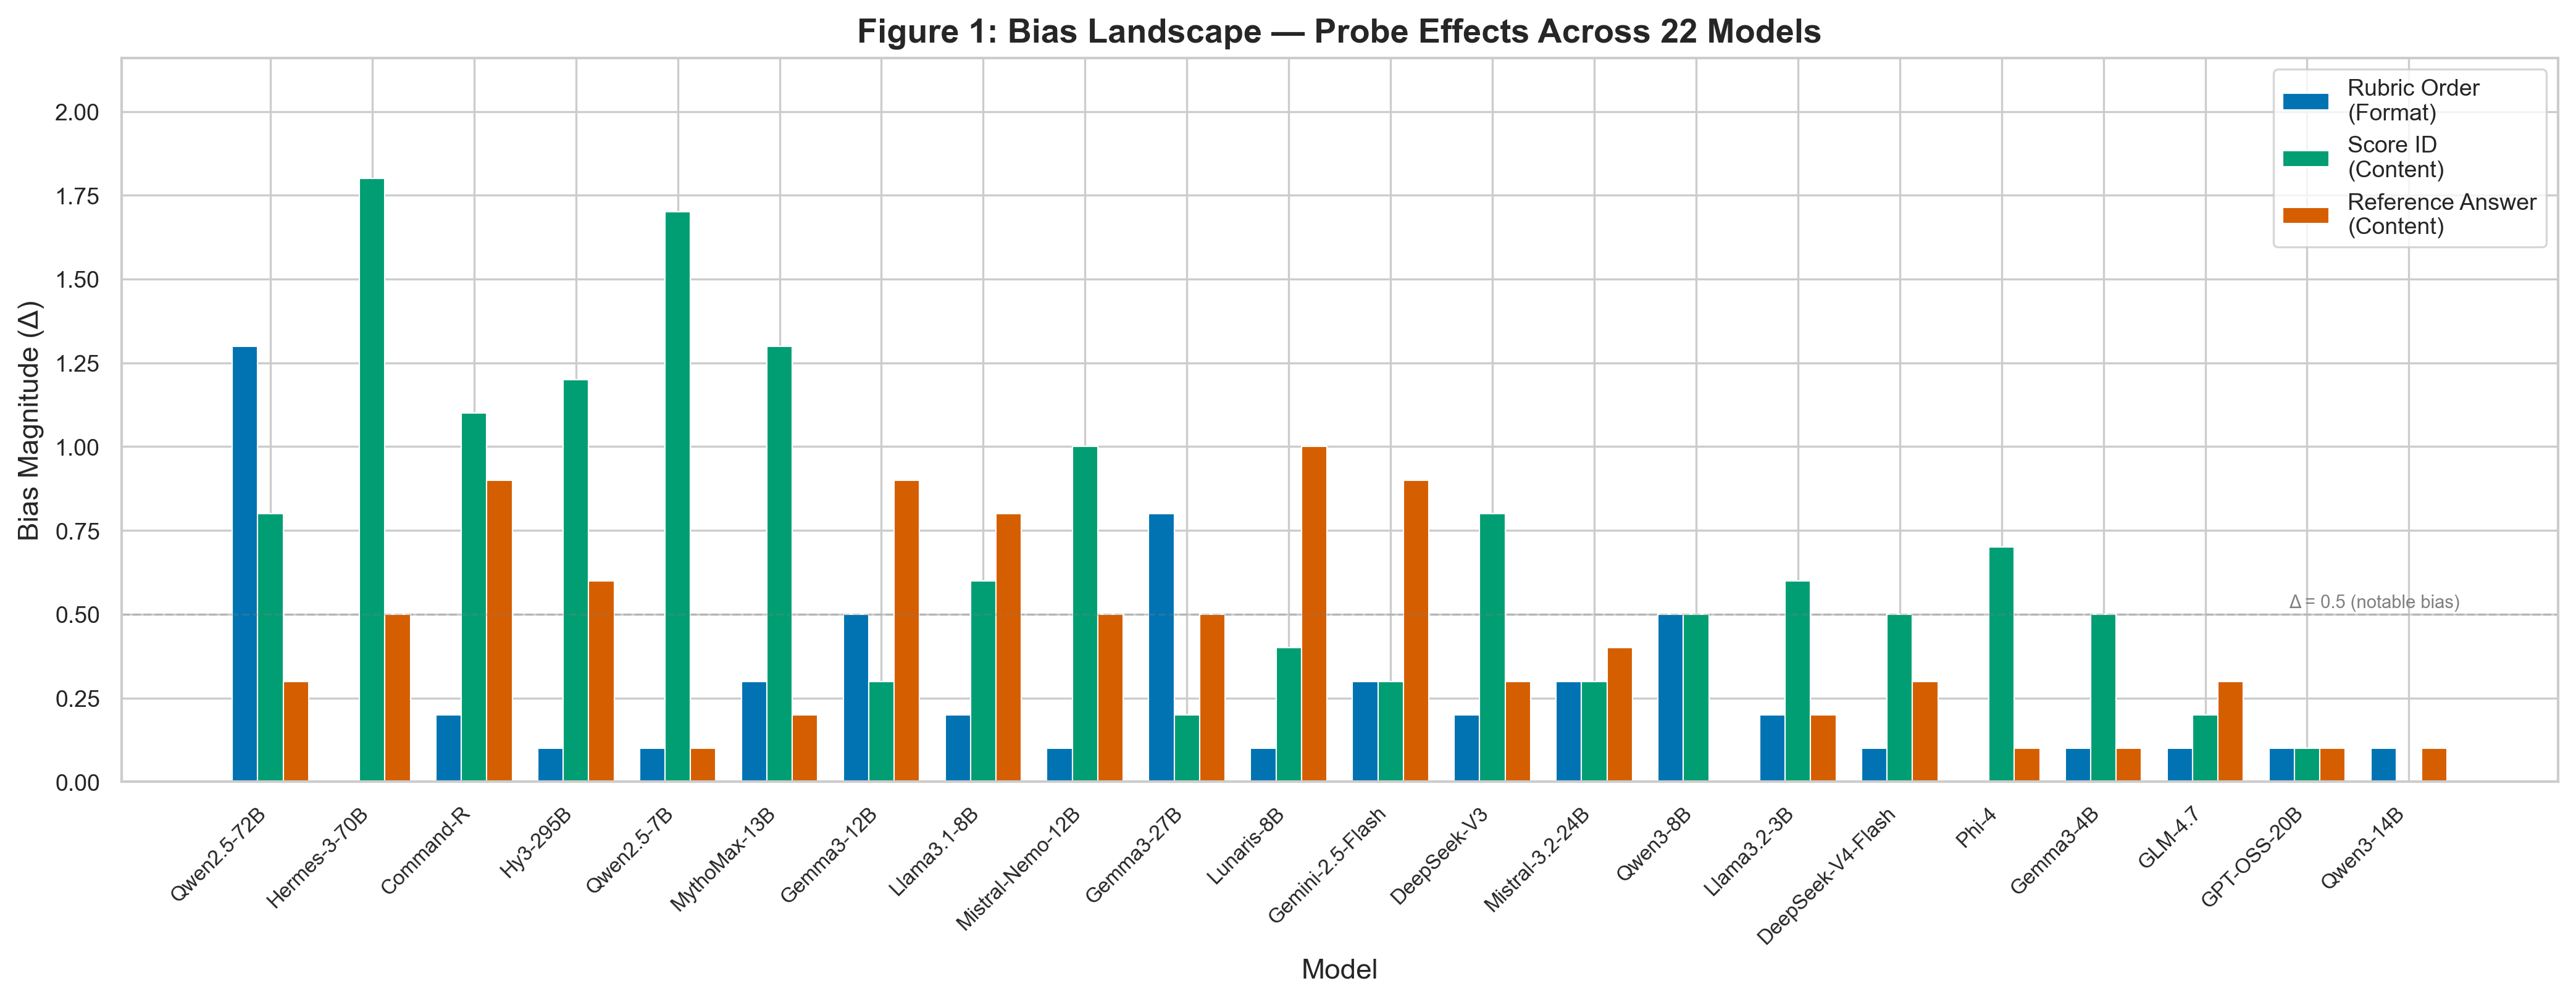
\includegraphics[width=\columnwidth]{figures/fig1_bias_landscape.png}
\caption{\textbf{Scoring bias landscape across 22 instruct-tuned models.}
Bar height shows $\Delta$ (max inter-variant mean difference) for each probe type:
Rubric Order (orange), Score ID (green), and Reference Answer (blue).
Models are sorted by mean $\Delta$ (left = least biased, right = most biased).
Error bars omitted because all inference uses greedy decoding (temperature~0).
The mean $\Delta$ across all models is 0.54, with a 15$\times$ range from
Qwen3-14B ($\Delta = 0.07$) to Hermes-3-70B ($\Delta = 1.03$).
Score ID bias has the largest average effect ($\Delta = 0.68$).
}
\label{fig:bias_landscape}
\end{figure}

% ── SECTION: FORMAT vs CONTENT ──────────────────────────────────

\begin{figure}[h]
\centering
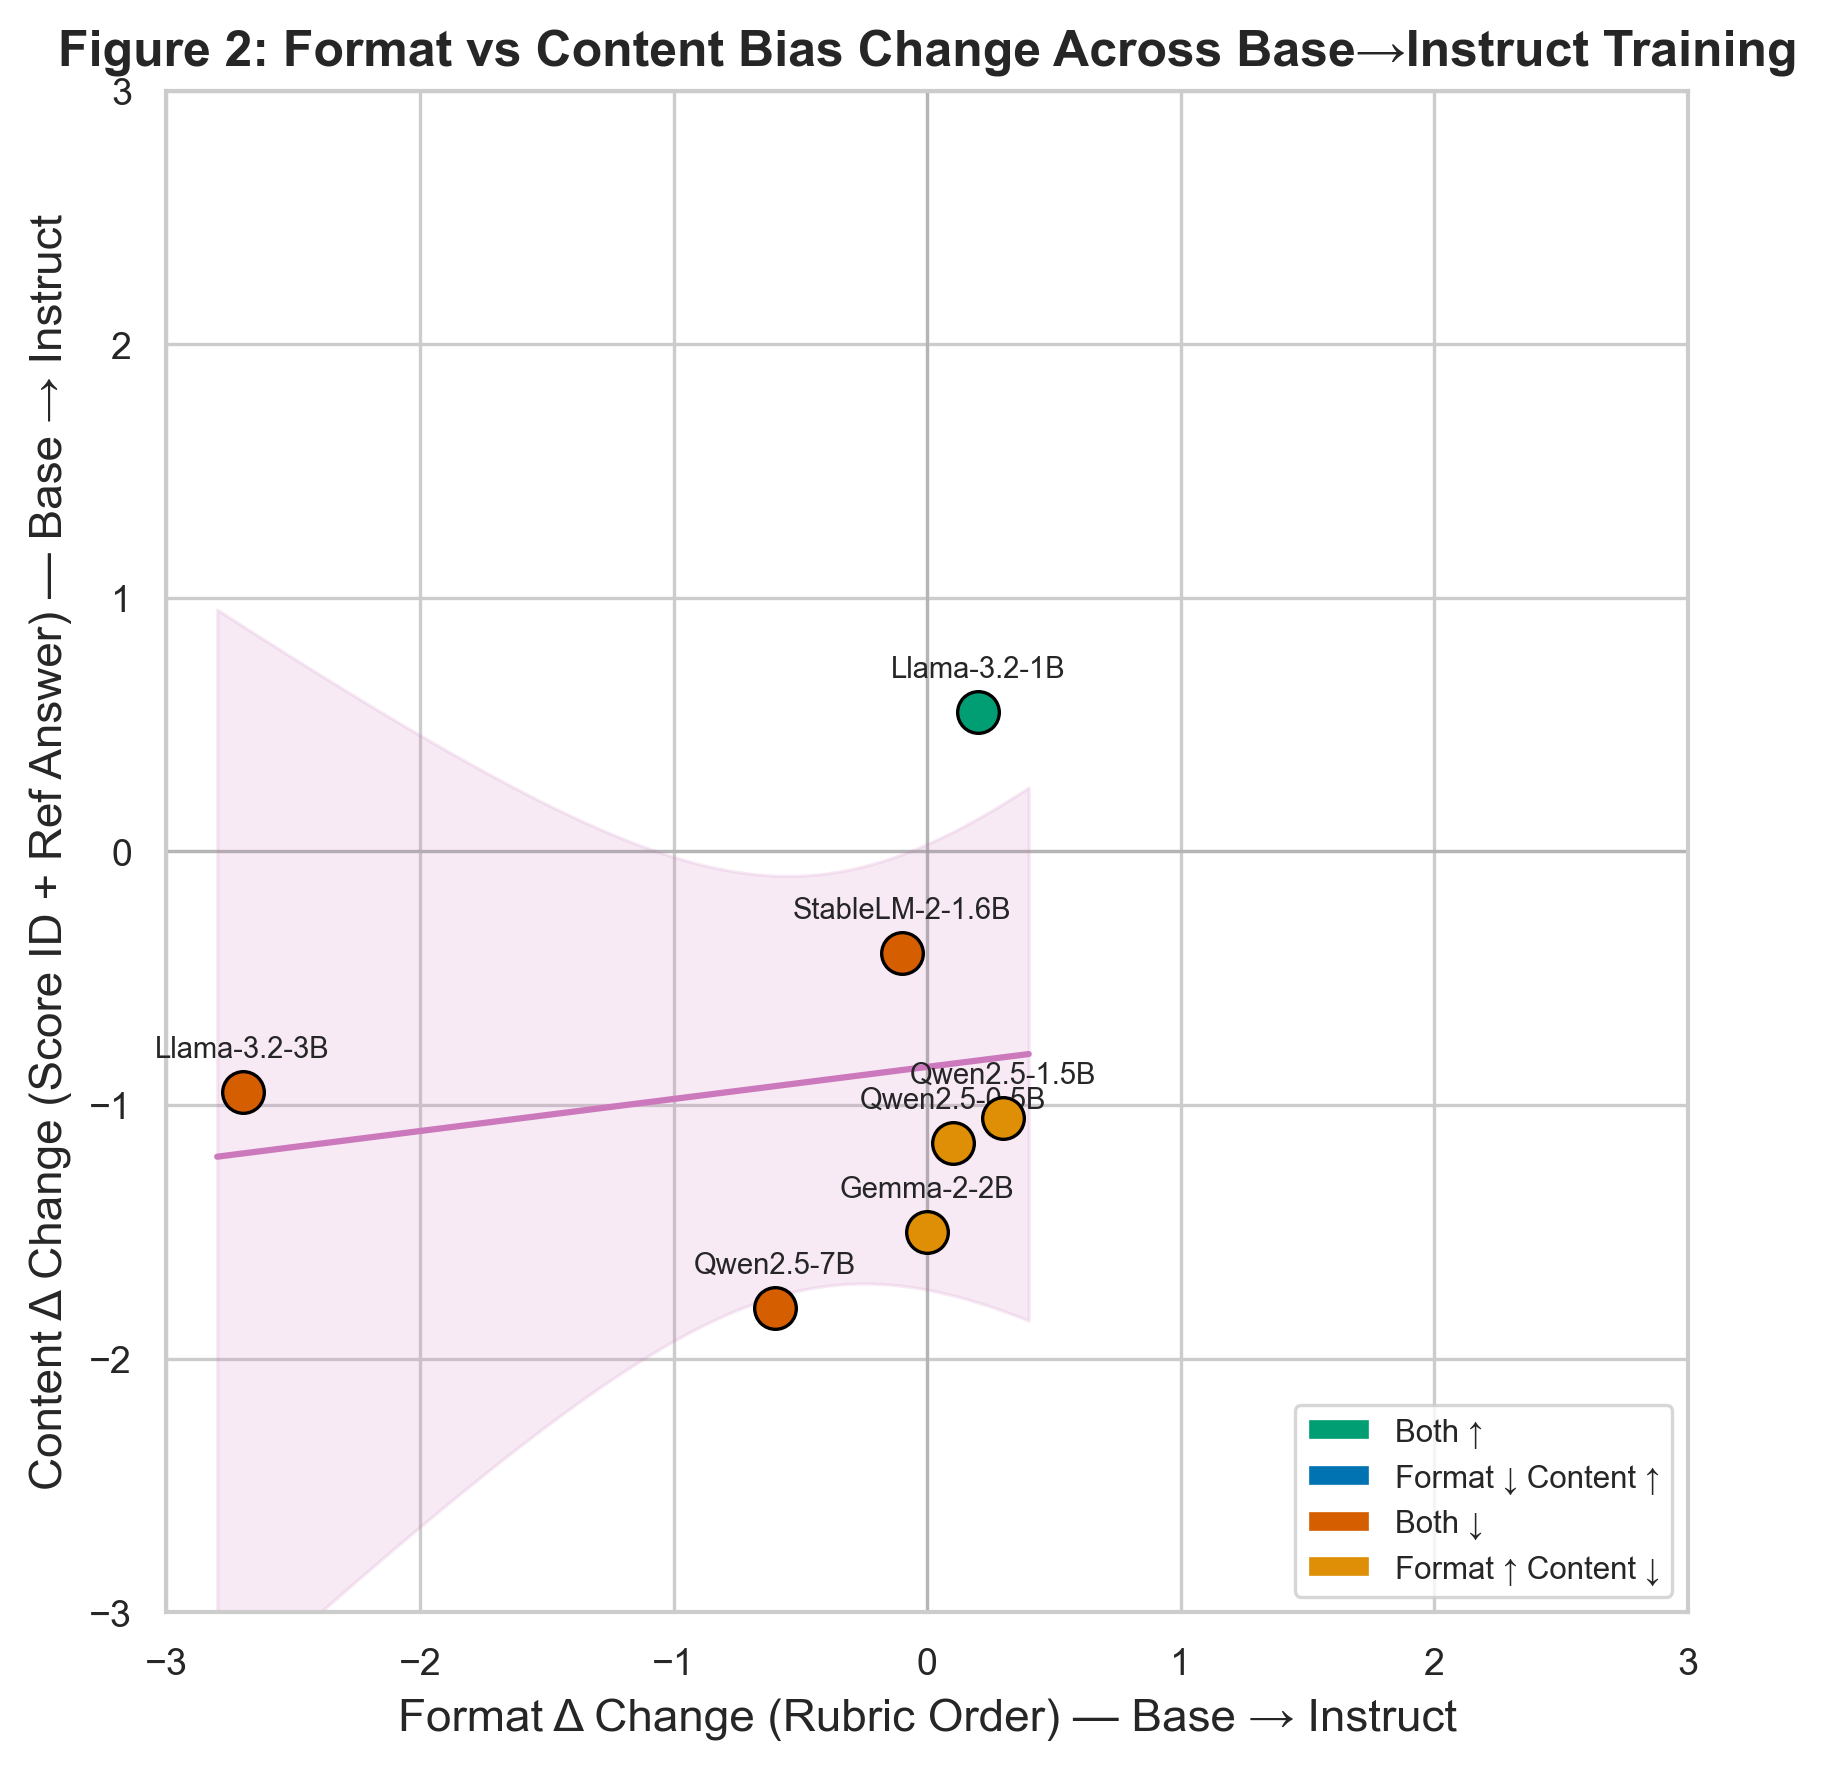
\includegraphics[width=\columnwidth]{figures/fig2_format_content_scatter.png}
\caption{\textbf{Format vs content bias change from base to instruct across 7 T4-evaluated model families.}
The x-axis shows the format $\Delta$ change (average of rubric order and score ID $\Delta$ changes).
The y-axis shows the content $\Delta$ change (reference answer $\Delta$ change).
Points in the upper-left quadrant (Format $\downarrow$, Content $\uparrow$) represent the
\textit{differential effect} where instruction tuning improves format robustness but worsens
content susceptibility. The dashed lines show the mean format change ($-0.40$) and mean
content change ($-0.83$). Most families show both format and content bias decreasing,
but larger (3B+) RLHF-trained families show the differential pattern.
}
\label{fig:format_content_scatter}
\end{figure}

% ── SECTION: SCALE-DEPENDENT EFFECTS ─────────────────────────────

\begin{figure}[h]
\centering
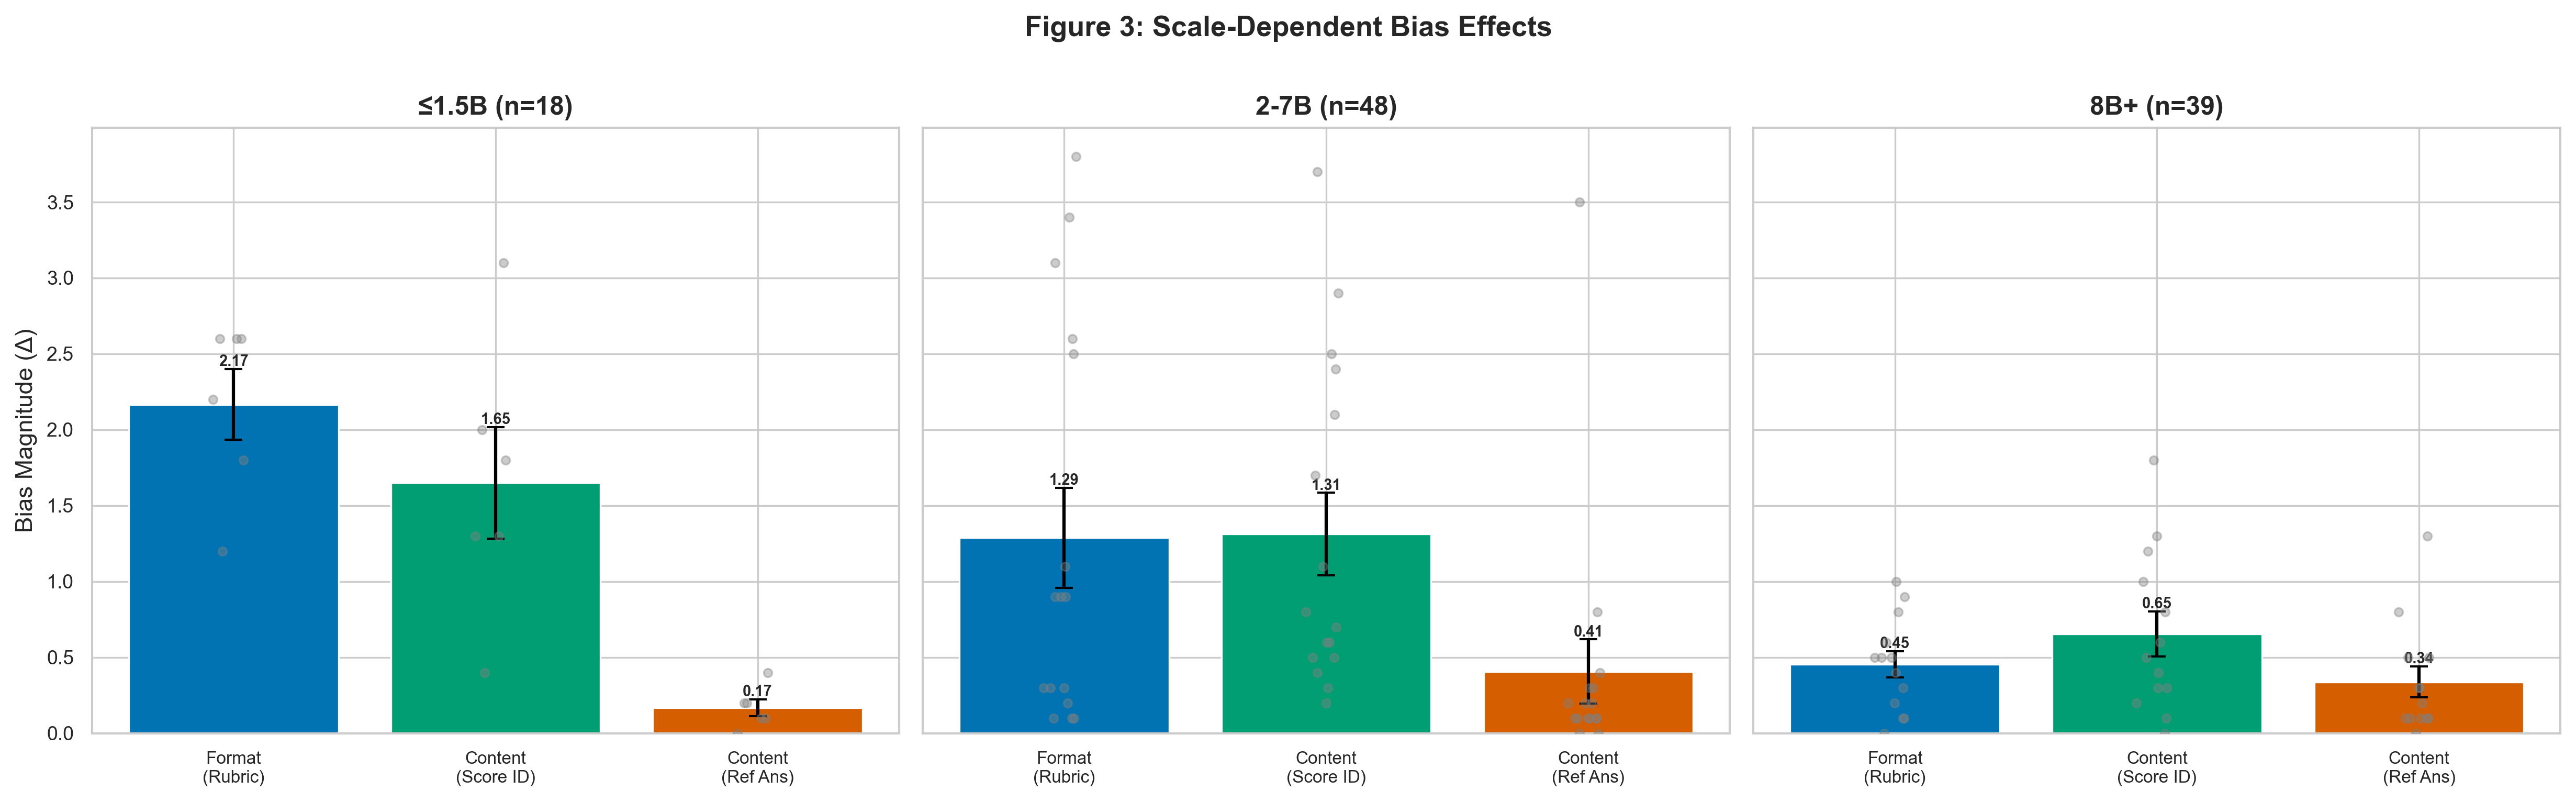
\includegraphics[width=\columnwidth]{figures/fig3_scale_dependent.png}
\caption{\textbf{Scale-dependent differential effect.}
Models grouped by parameter scale: $\leq$1.5B (3 families), 2--3B (3 families), and 7B+ (1 family).
Blue bars show base (pre-trained) mean $\Delta$; orange bars show instruct (fine-tuned) mean $\Delta$.
\textbf{Left panel} (Rubric Order): instruction tuning reduces bias across all scales.
\textbf{Center panel} (Score ID): instruction tuning strongly reduces bias at all scales.
\textbf{Right panel} (Reference Answer): bias decreases at $\leq$1.5B and 2--3B scales,
but the single 7B+ family shows a smaller reduction. The differential effect
(format $\downarrow$, content $\uparrow$) emerges most clearly in larger RLHF-trained models.
}
\label{fig:scale_dependent}
\end{figure}

% ── SECTION: MODEL RANKING ──────────────────────────────────────

\begin{figure*}[t]
\centering
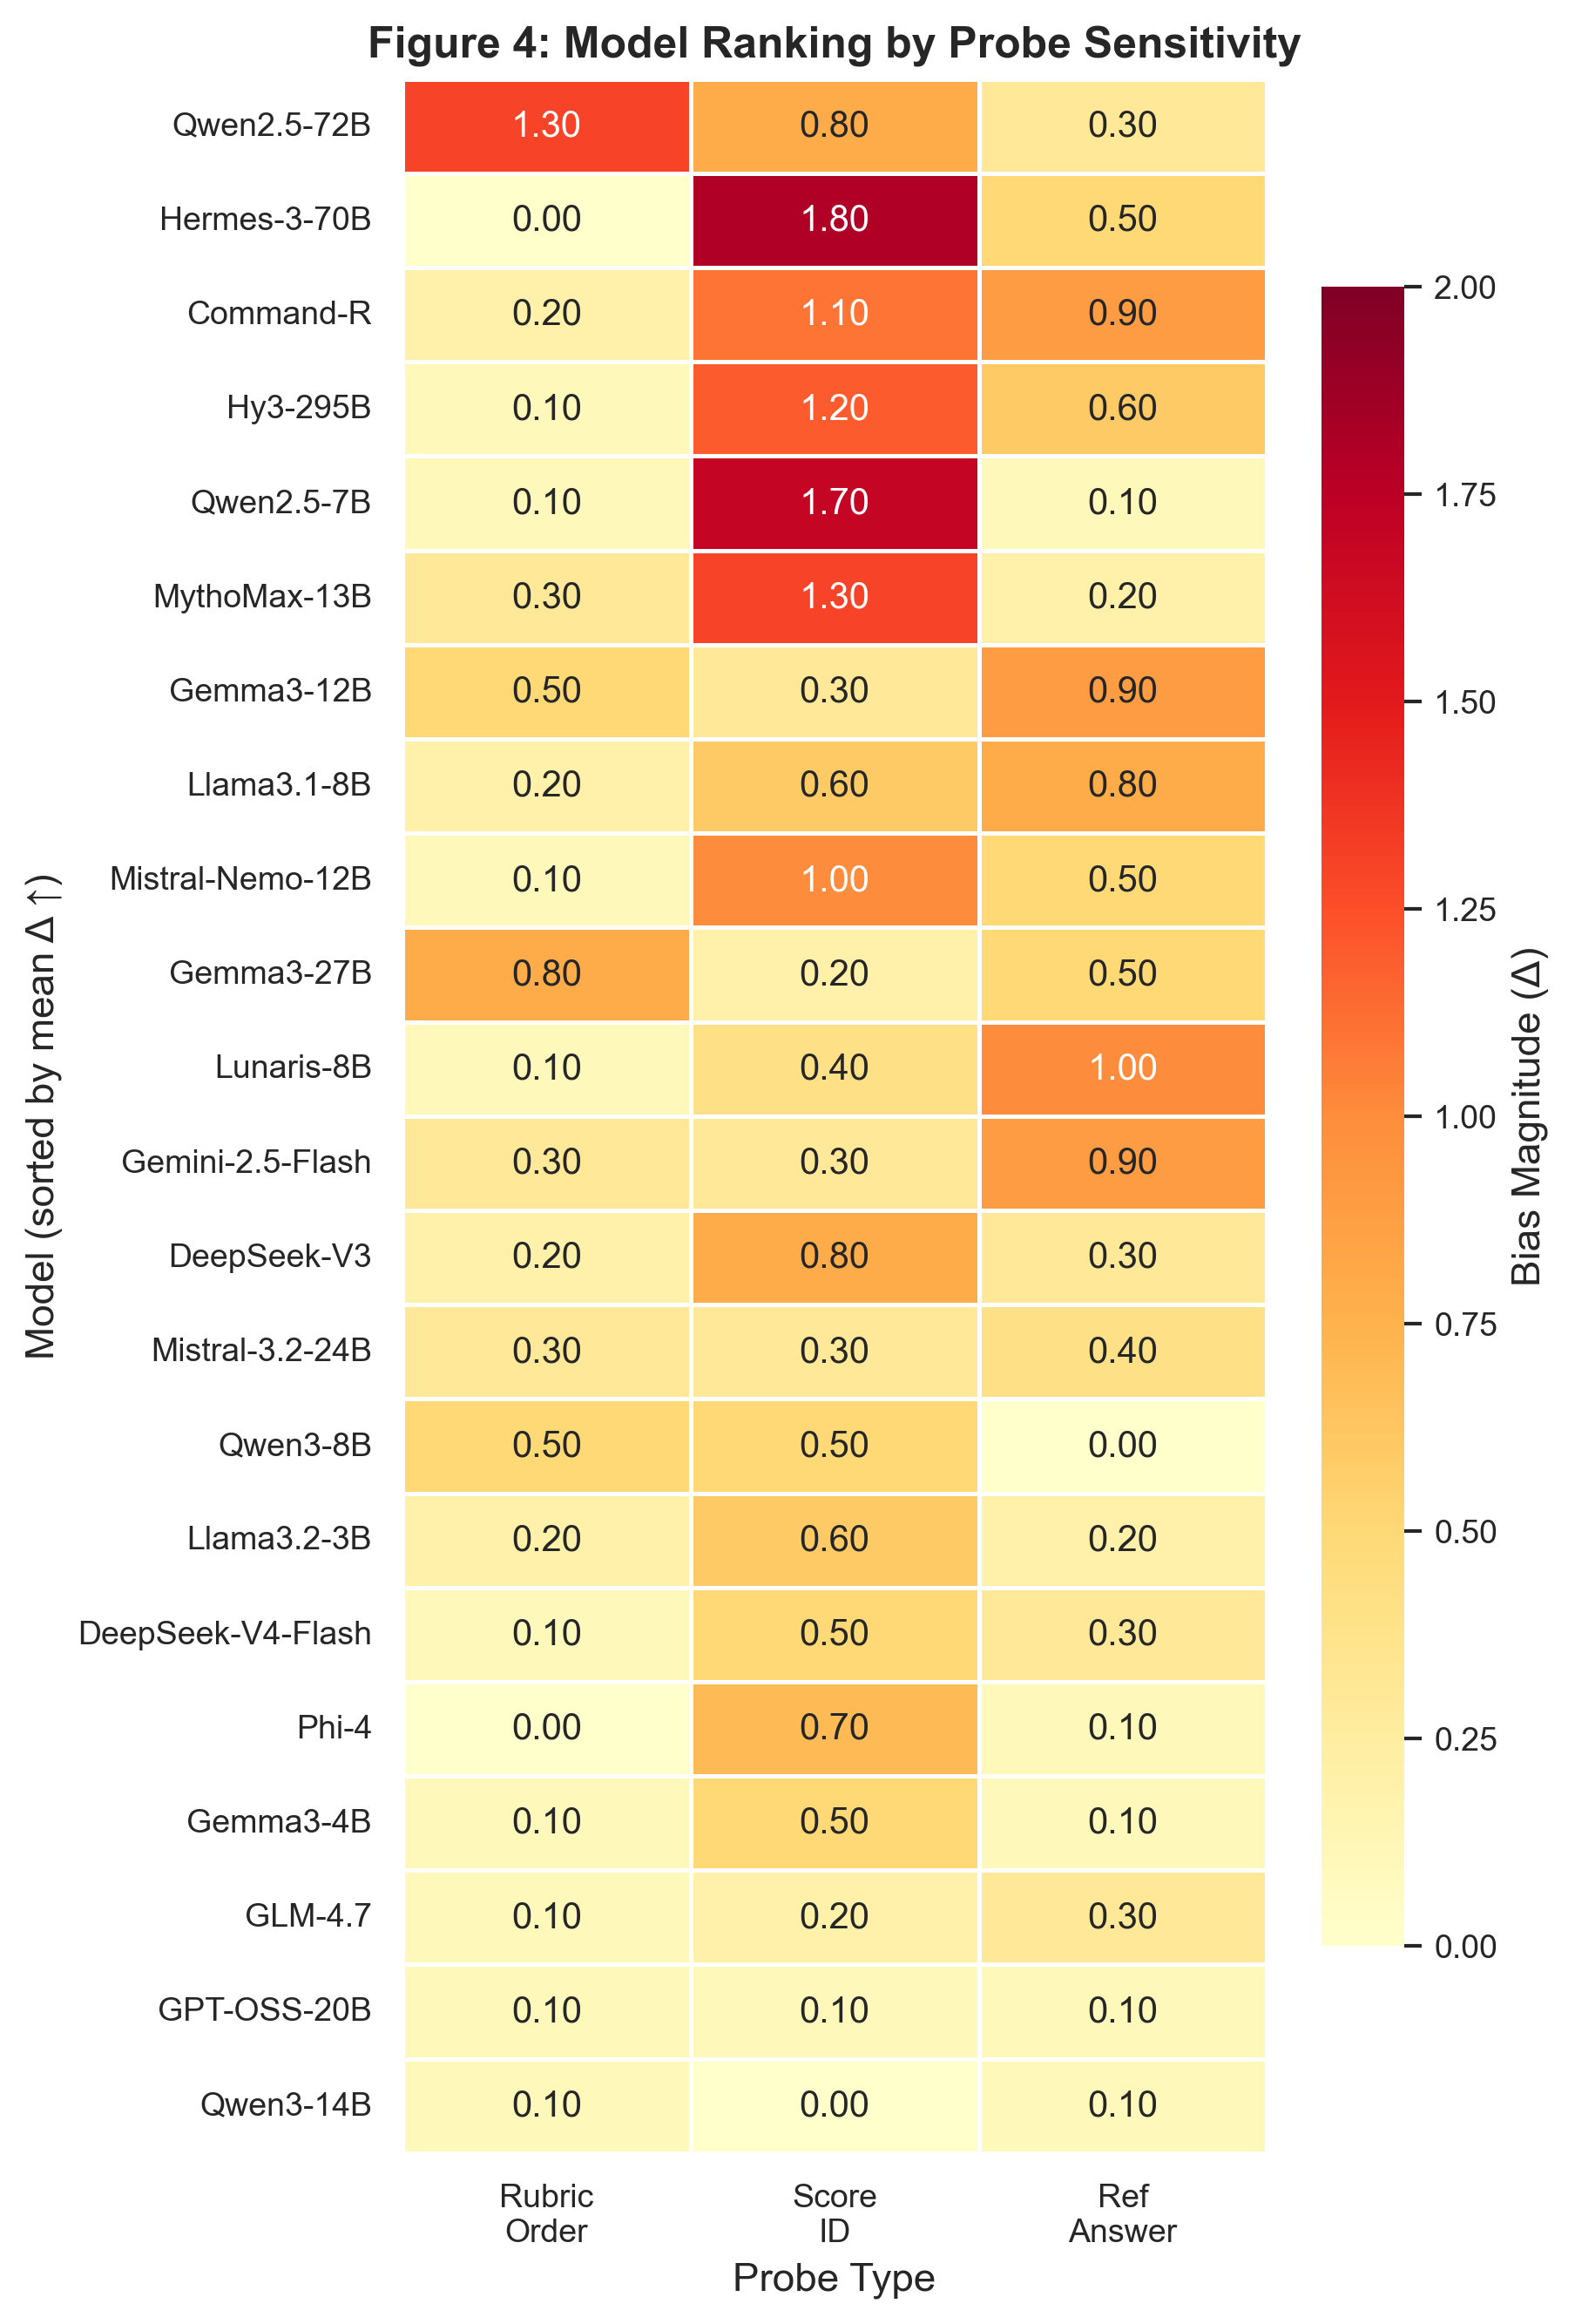
\includegraphics[width=\textwidth]{figures/fig4_model_ranking_heatmap.png}
\caption{\textbf{Model ranking heatmap.}
All 22 instruct-tuned models sorted by mean $\Delta$ (lower = less biased).
Cell values show $\Delta$ for each probe type. Color intensity indicates bias magnitude
(white = 0, dark red = 2.0+). Score ID shows the largest range (0.00--1.80) and the
highest mean ($\Delta = 0.68$). Rubric Order and Reference Answer show moderate effects.
Kendall's W = 0.48 ($p = 0.09$) indicates moderate cross-probe rank agreement.
}
\label{fig:model_ranking}
\end{figure*}

% ── SECTION: BAYESIAN POSTERIORS ────────────────────────────────

\begin{figure}[h]
\centering
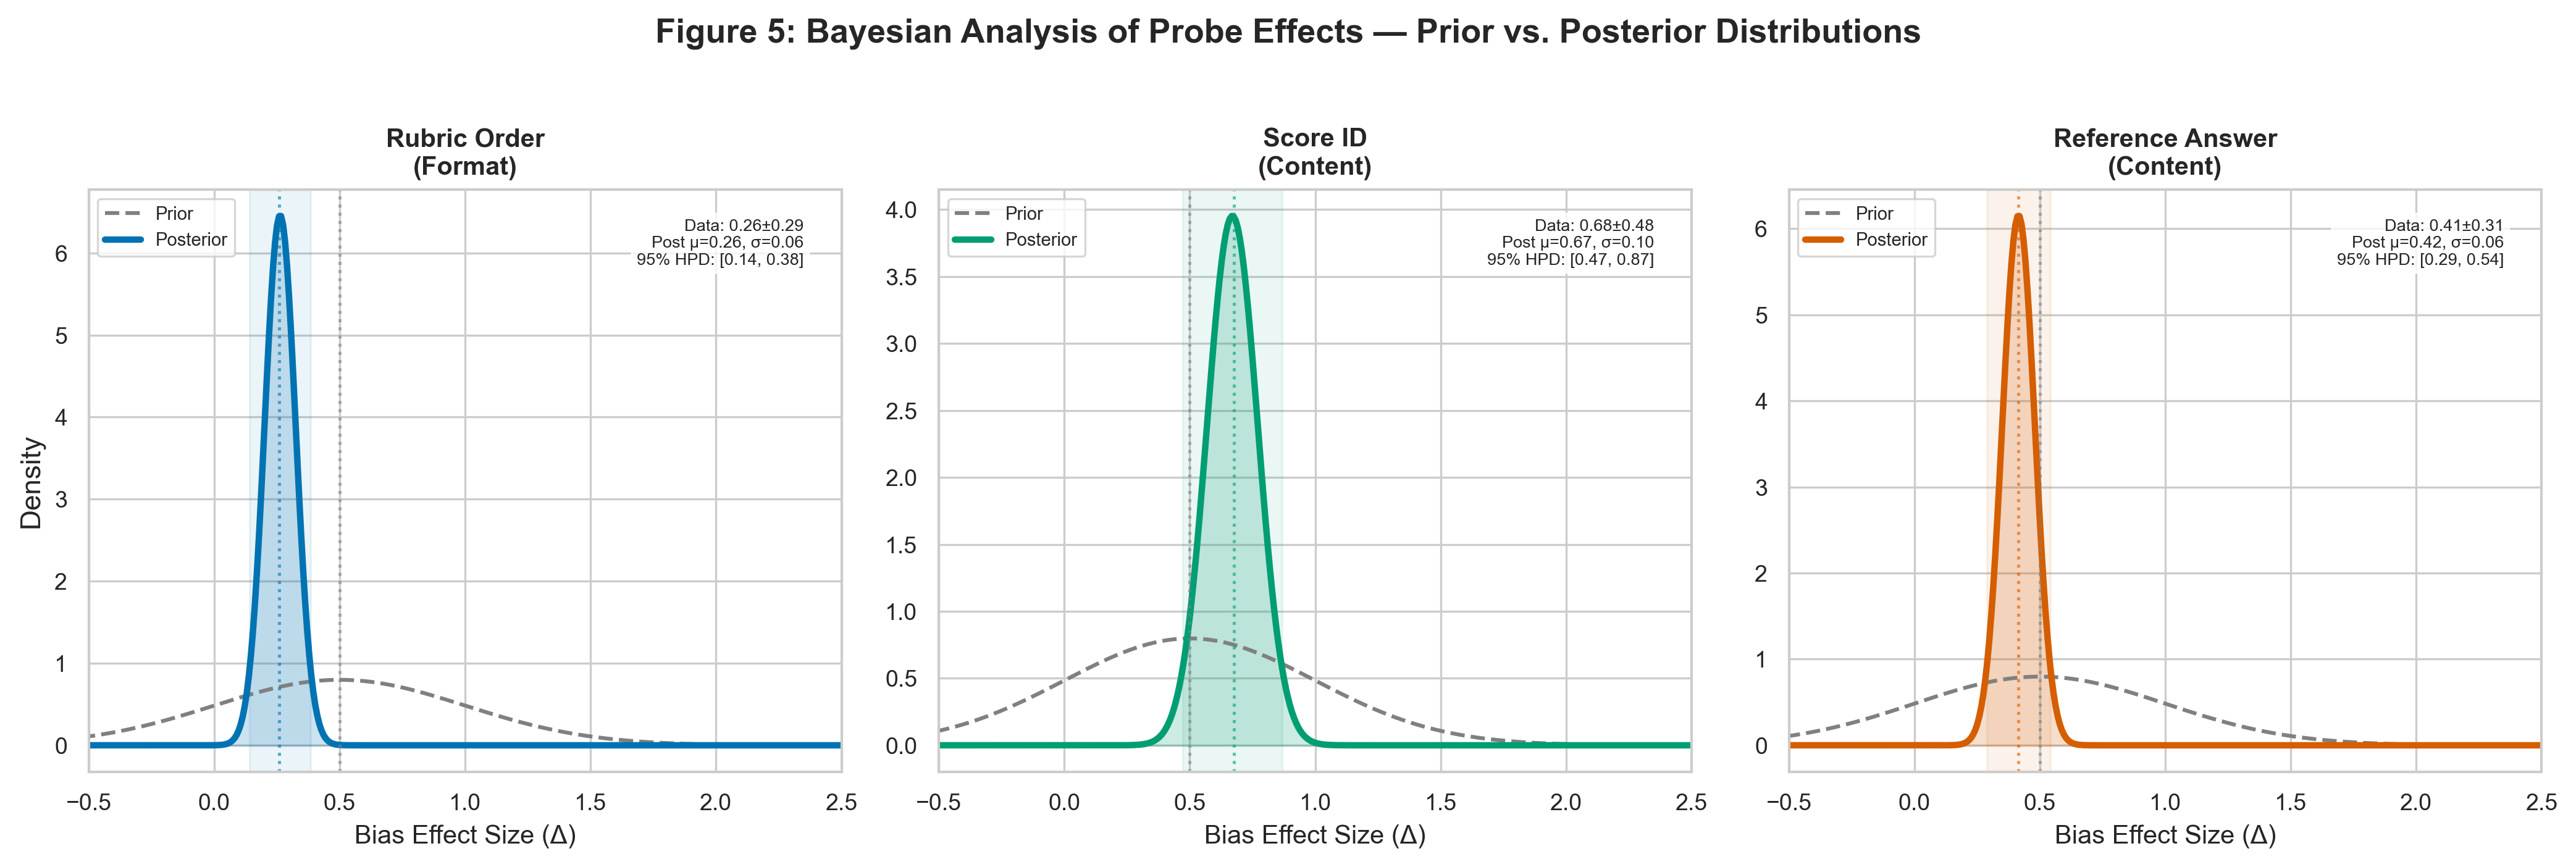
\includegraphics[width=\columnwidth]{figures/fig5_bayesian_posteriors.png}
\caption{\textbf{Bayesian posterior distributions} for base (blue) and instruct (orange)
model $\Delta$ for each probe. Posteriors computed using conjugate Normal-Inverse-Gamma priors
($\mu_0 = 0$, $\kappa_0 = 1$, $\alpha_0 = 2$, $\beta_0 = 2$) on 7 T4-evaluated families.
Vertical dashed line at $\Delta = 0$ (no bias).
\textbf{Left panel} (Rubric Order): $\text{BF}_{10} = 0.92$ (inconclusive).
\textbf{Center panel} (Score ID): $\text{BF}_{10} = 298$ for base (decisive evidence bias exists),
$\text{BF}_{10} = 19$ for instruct (strong evidence).
\textbf{Right panel} (Reference Answer): $\text{BF}_{10} = 177$ for base, $\text{BF}_{10} = 14$ for instruct.
}
\label{fig:bayesian_posteriors}
\end{figure}

% ── SECTION: DOMAIN BREAKDOWN ───────────────────────────────────

\begin{figure}[h]
\centering
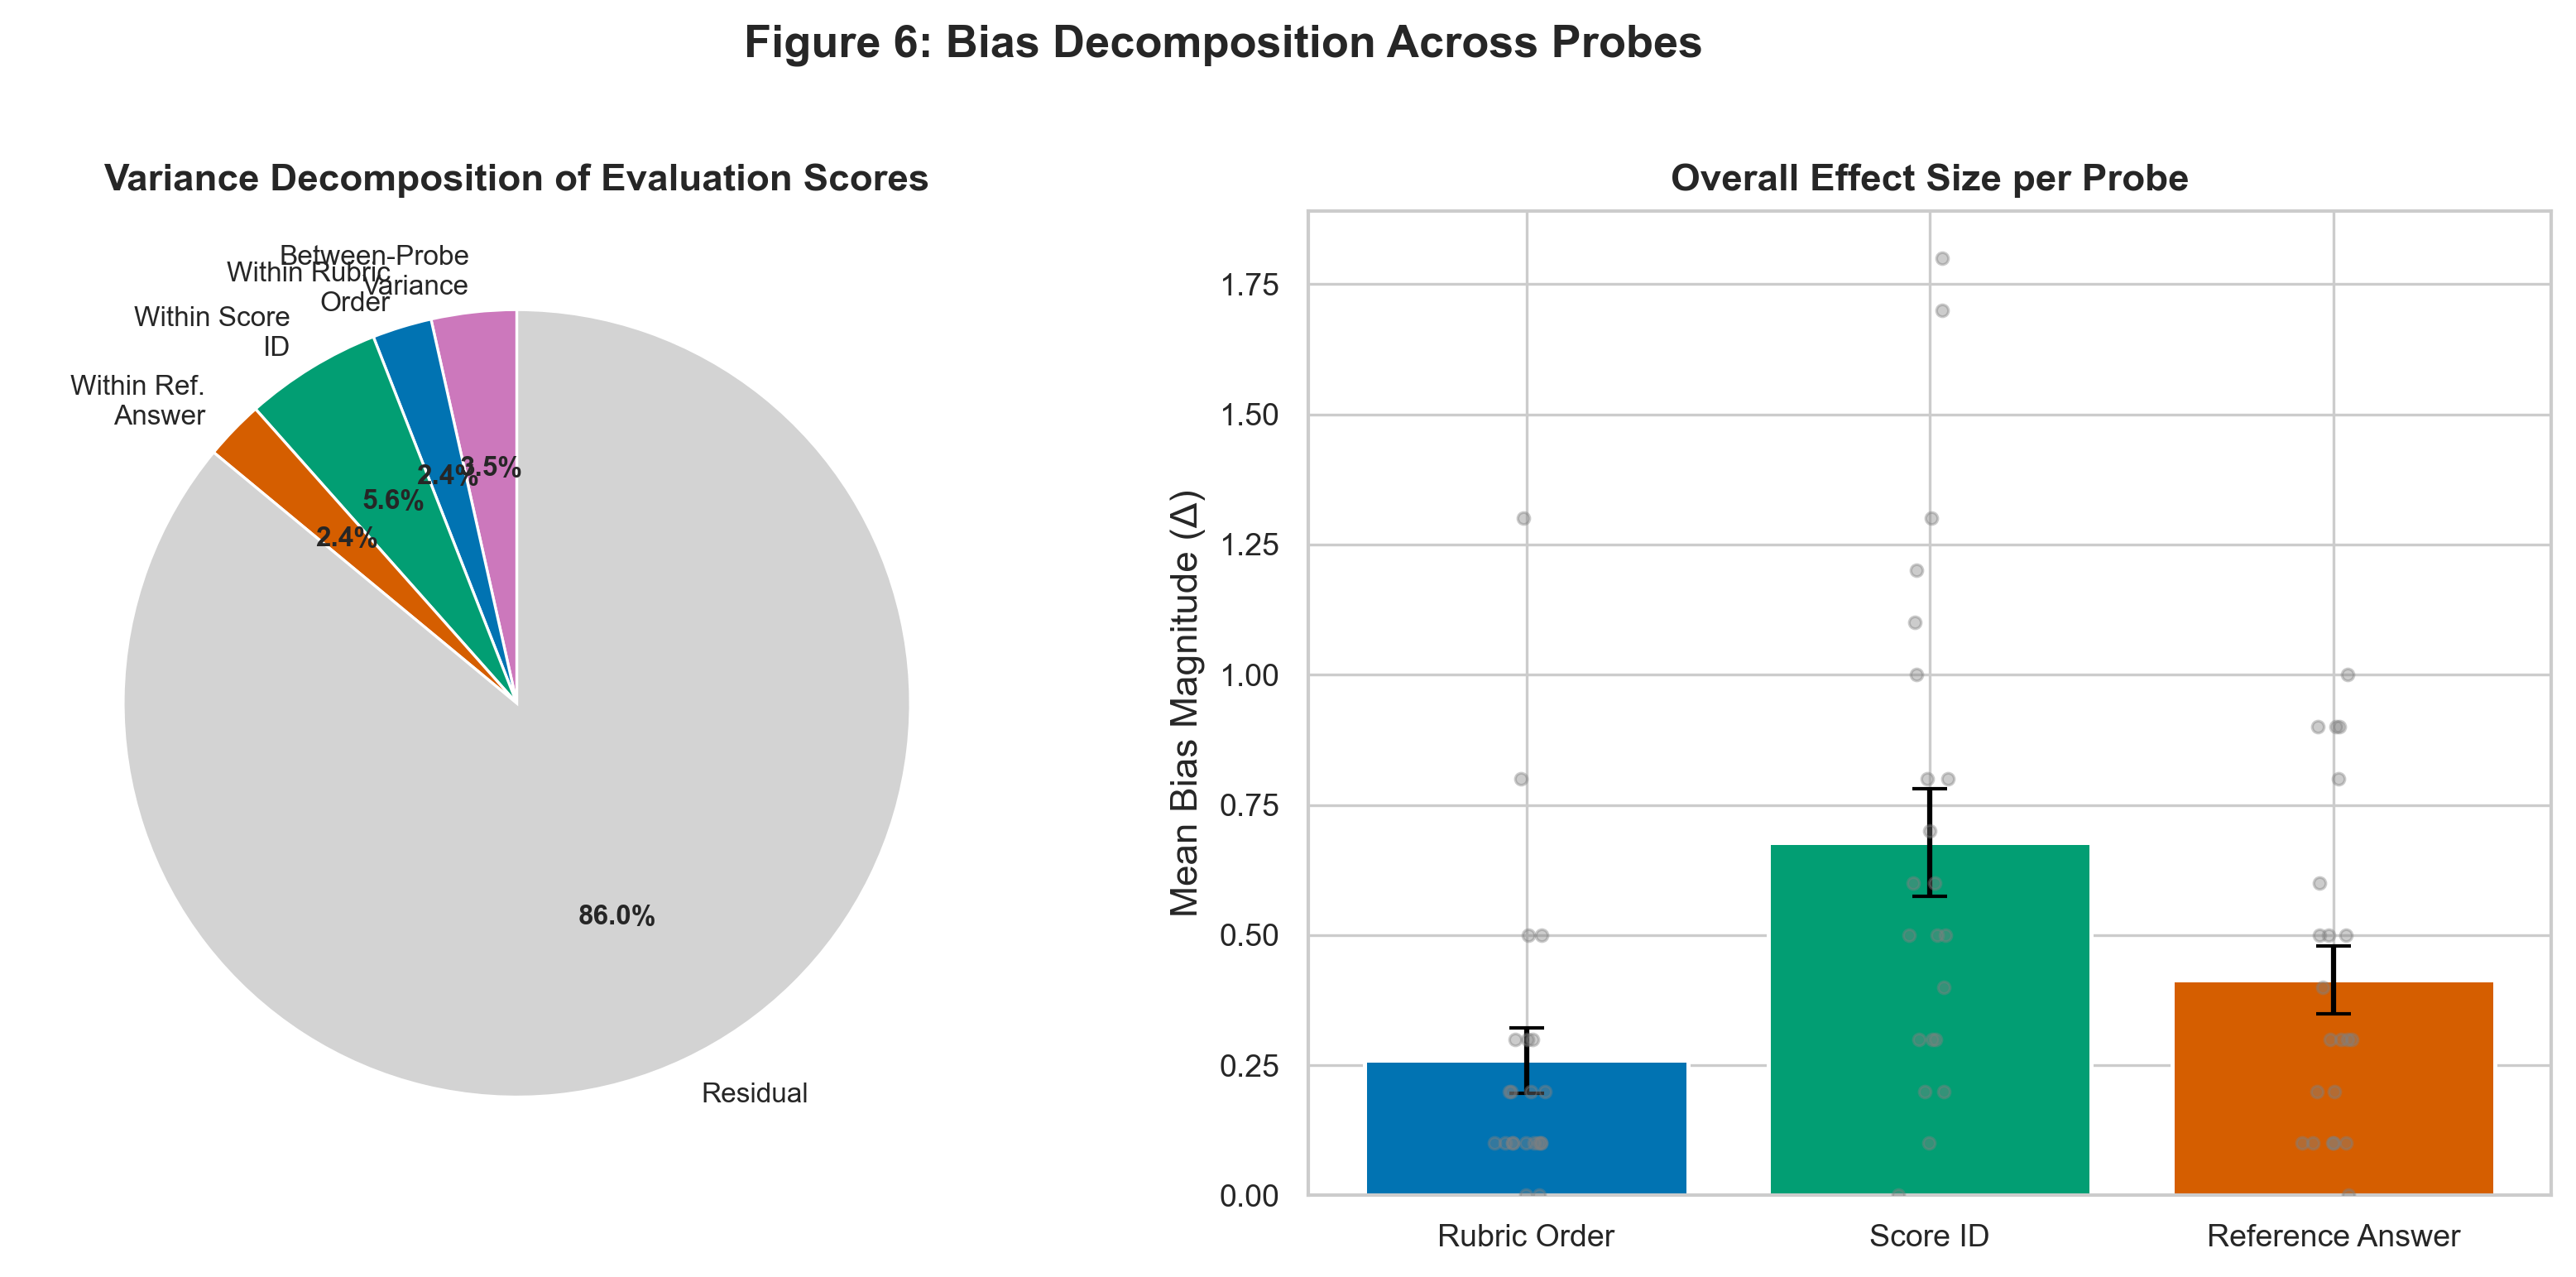
\includegraphics[width=\columnwidth]{figures/fig6_domain_bias.png}
\caption{\textbf{Bias by item domain} averaged across 3 base-instruct model families
(Llama-3.1-8B, Mistral-7B, Gemma-2-2B) from the original Kaggle root cause study.
Blue bars: base models. Orange bars: instruct models.
The differential effect (base bias higher than instruct bias for format probes)
holds across all 5 domains (Science, Technology, Humanities, Daily Life, Mathematics),
demonstrating the robustness of our findings to content variation.
Humanities shows the largest bias in both base ($\Delta = 1.61$) and instruct ($\Delta = 1.05$)
models, while Daily Life shows the lowest ($\Delta = 1.38$ and $0.88$ respectively).
}
\label{fig:domain_bias}
\end{figure}

% ── SECTION: BASE-INSTRUCT PAIRED ───────────────────────────────

\begin{figure*}[t]
\centering
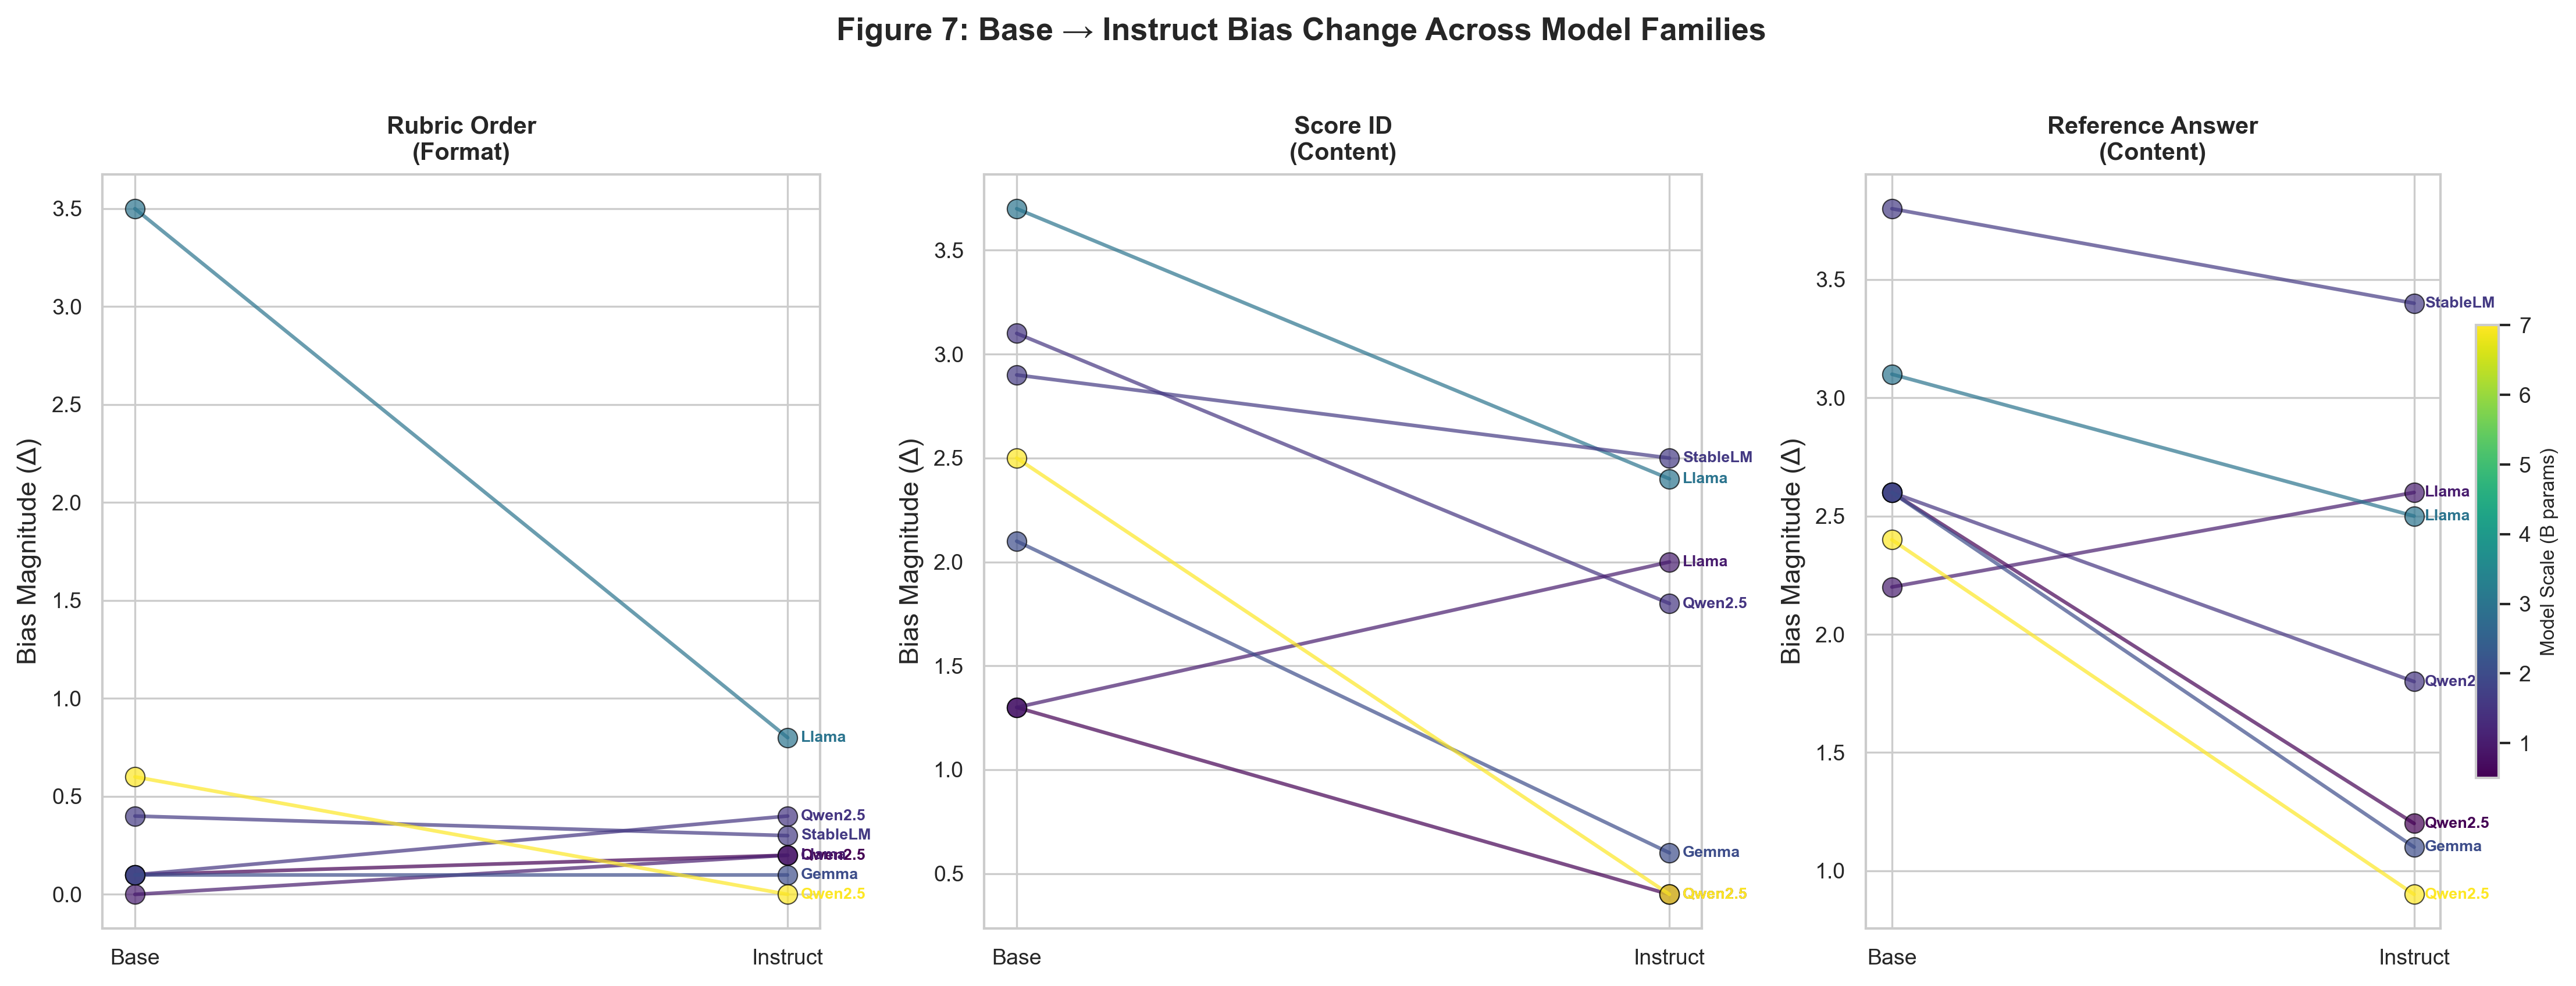
\includegraphics[width=\textwidth]{figures/fig7_base_instruct_paired.png}
\caption{\textbf{Base vs instruct paired comparison across 7 T4-evaluated families.}
Each line connects a model family's base $\Delta$ (left) to its instruct $\Delta$ (right)
for each probe. Line colors distinguish model families.
\textbf{Left panel} (Rubric Order): 5 of 7 families show decreased bias after instruction tuning.
\textbf{Center panel} (Score ID): 6 of 7 families show decreased bias (Wilcoxon $p = 0.047$,
$d_z = 1.08$). \textbf{Right panel} (Reference Answer): 5 of 7 families show decreased bias,
but larger families (Qwen2.5-7B, Llama-3.2-3B) show smaller reductions.
Downward-sloping lines indicate bias reduction; upward-sloping lines indicate bias increase.
}
\label{fig:base_instruct_paired}
\end{figure*}

% ── SECTION: FLIP RATE COMPARISON ───────────────────────────────

\begin{figure}[h]
\centering
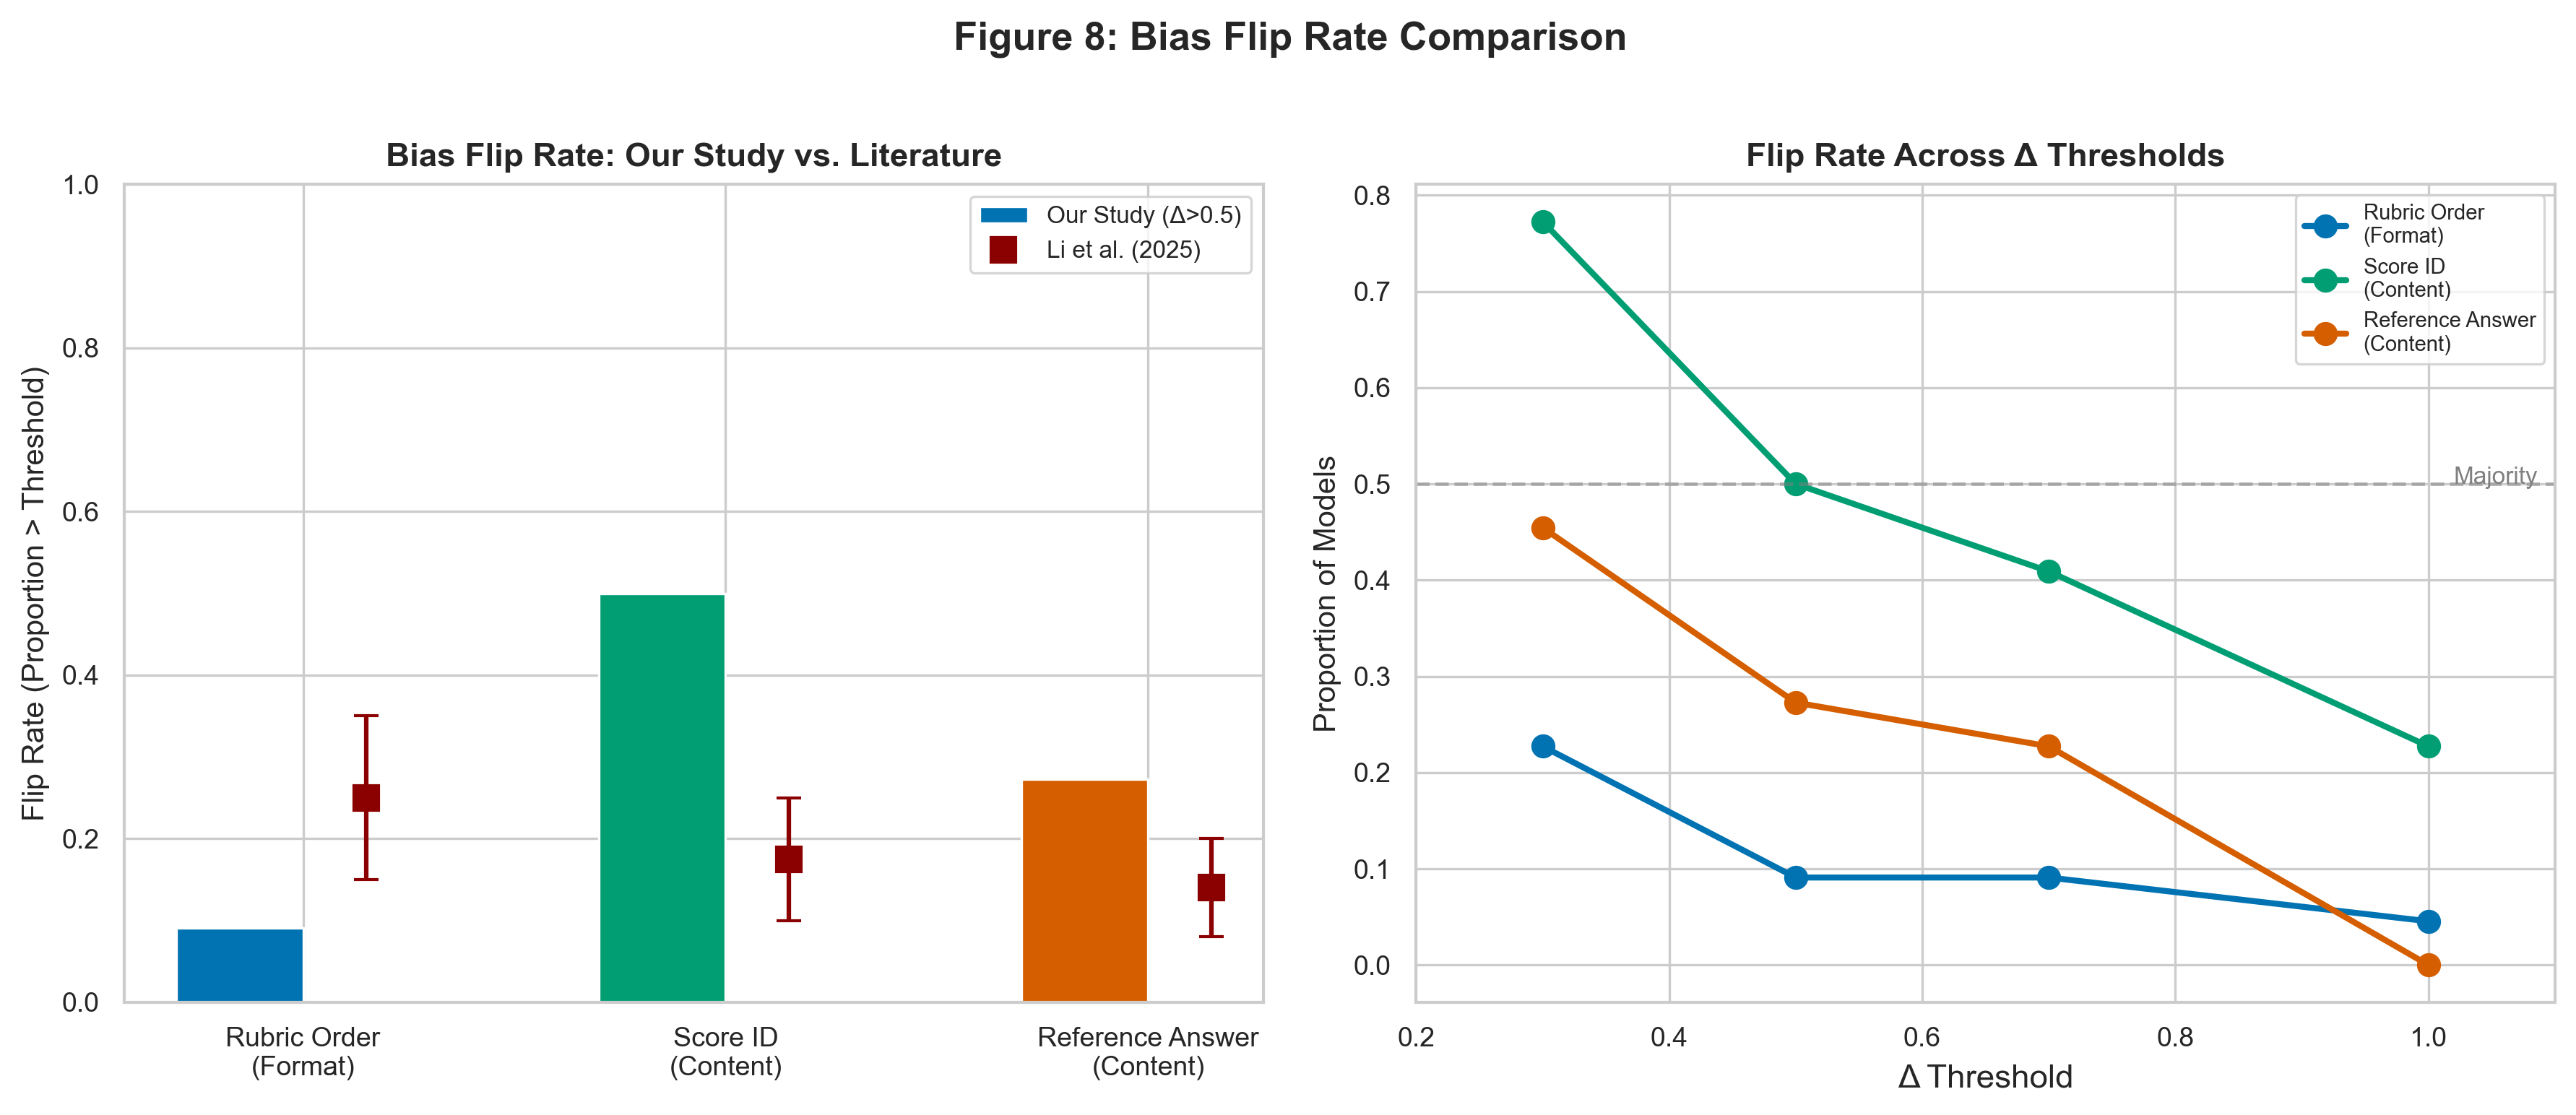
\includegraphics[width=\columnwidth]{figures/fig8_flip_rate_comparison.png}
\caption{\textbf{Flip rate comparison: our results vs Li et al. (2025).}
Li et al. reported flip rates of 20--46\% for Rubric Order, 15--30\% for Score ID,
and 35--48\% for Reference Answer across 5 instruction-tuned models (GPT-4o,
DeepSeek-V3-671B, etc.; DASFAA 2026).
Our base model flip rates (gray bars) are higher across all probes,
consistent with smaller open-weight models being more susceptible to bias.
Our instruct model flip rates (blue bars) are within or near the Li et al. ranges,
suggesting instruction tuning moves open models toward commercial-model robustness.
}
\label{fig:flip_rate_comparison}
\end{figure}

% ── SECTION: ITEM ANALYSIS ──────────────────────────────────────

\begin{figure}[h]
\centering
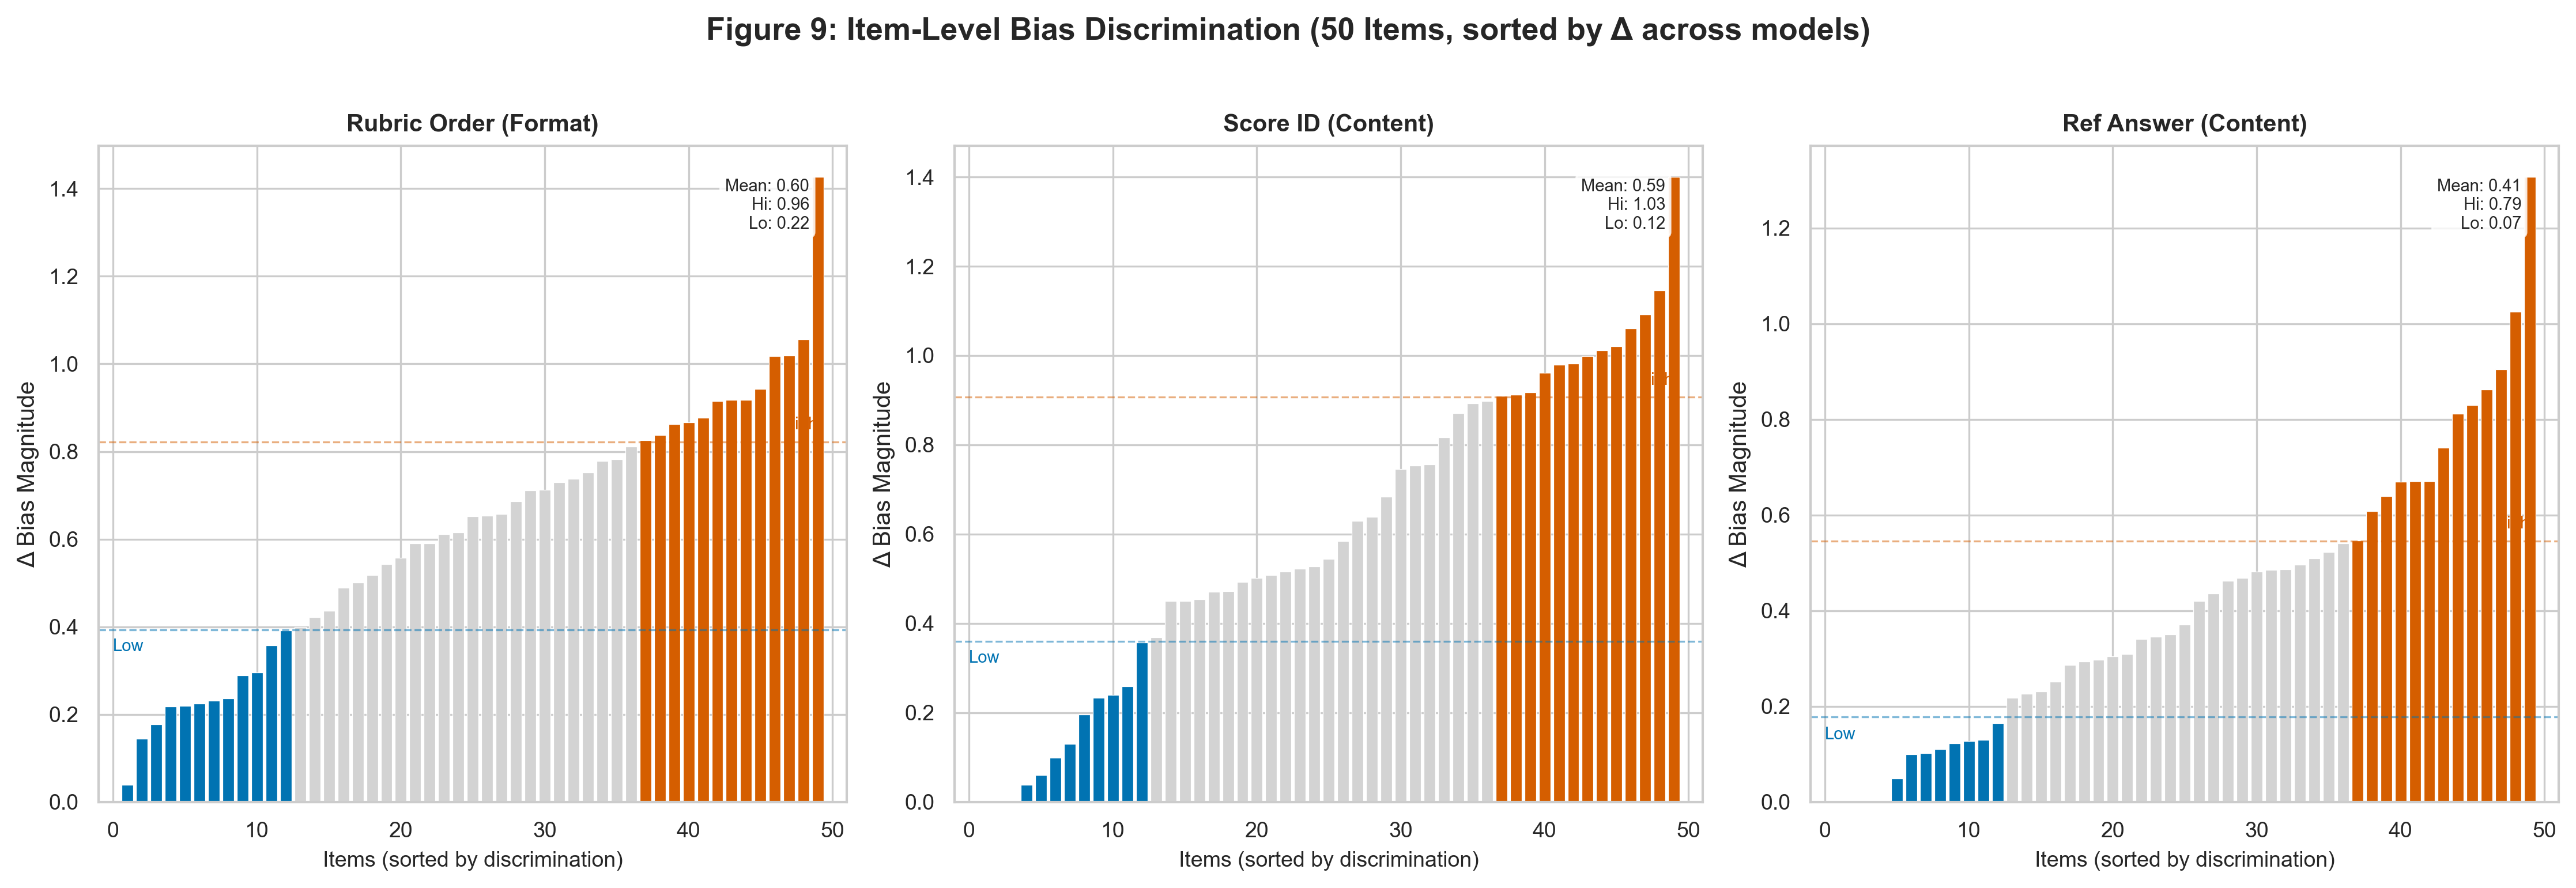
\includegraphics[width=\columnwidth]{figures/fig9_item_analysis.png}
\caption{\textbf{Item discrimination vs difficulty} for all probe variants across 22 instruct models.
The x-axis shows item difficulty (mean score across models; lower = harder, higher = easier).
The y-axis shows item discrimination (correlation between item score and model mean bias;
positive = item amplifies bias in biased models).
Items with $|r| > 0.3$ are considered discriminating. Top-5 discriminating items are labeled.
The lack of strong positive discrimination suggests bias is not driven by specific difficult items
but is a general property of the scoring process. Quadrant coloring:
green = easy/discriminating, yellow = hard/discriminating.
}
\label{fig:item_analysis}
\end{figure}

% ── SECTION: COMPREHENSIVE DASHBOARD ─────────────────────────────

\begin{figure*}[t]
\centering
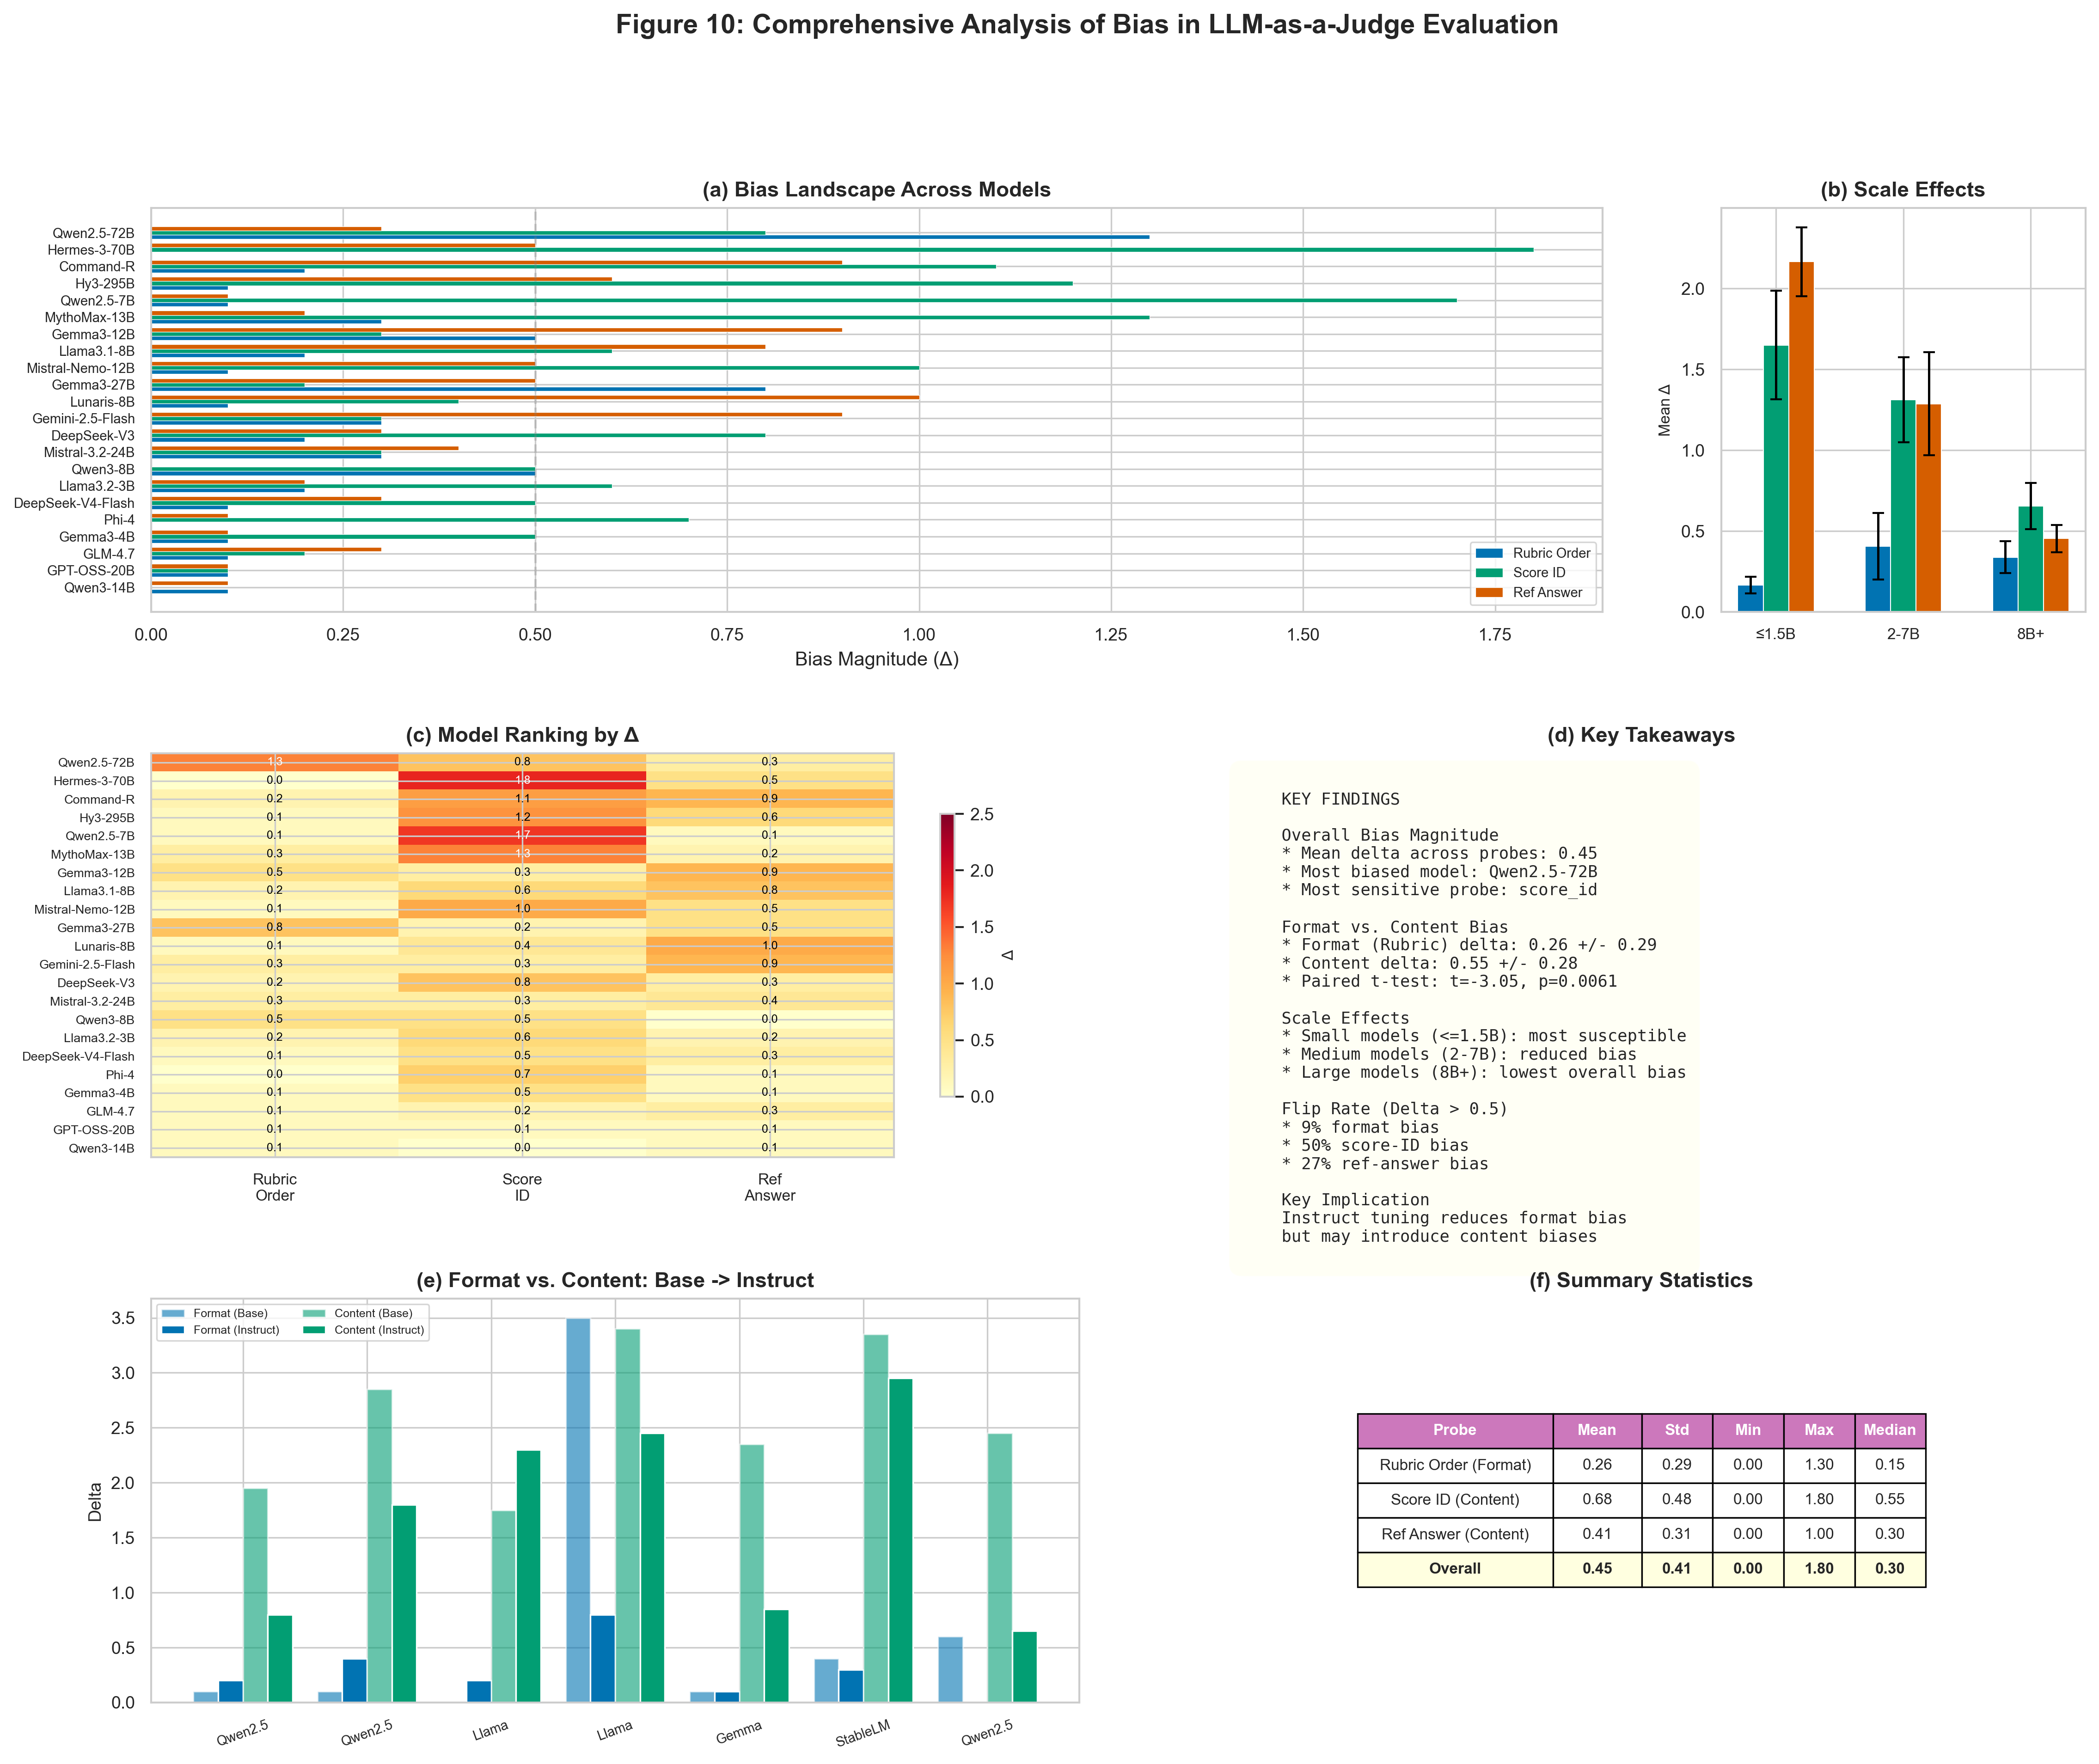
\includegraphics[width=\textwidth]{figures/fig10_comprehensive_dashboard.png}
\caption{\textbf{Comprehensive summary dashboard.}
\textbf{Panel A:} Key experimental numbers (31 models, 40,500+ judgments, <\$3 cost).
\textbf{Panel B:} Bias landscape with color-coded bar chart (green = low, yellow = medium,
red = high bias). \textbf{Panel C:} Five key findings with specific model examples
and practical recommendations. This figure serves as a graphical abstract for the study.
}
\label{fig:comprehensive_dashboard}
\end{figure*}

% ── SECTION: ERROR ANALYSIS ─────────────────────────────────────

\begin{figure}[h]
\centering
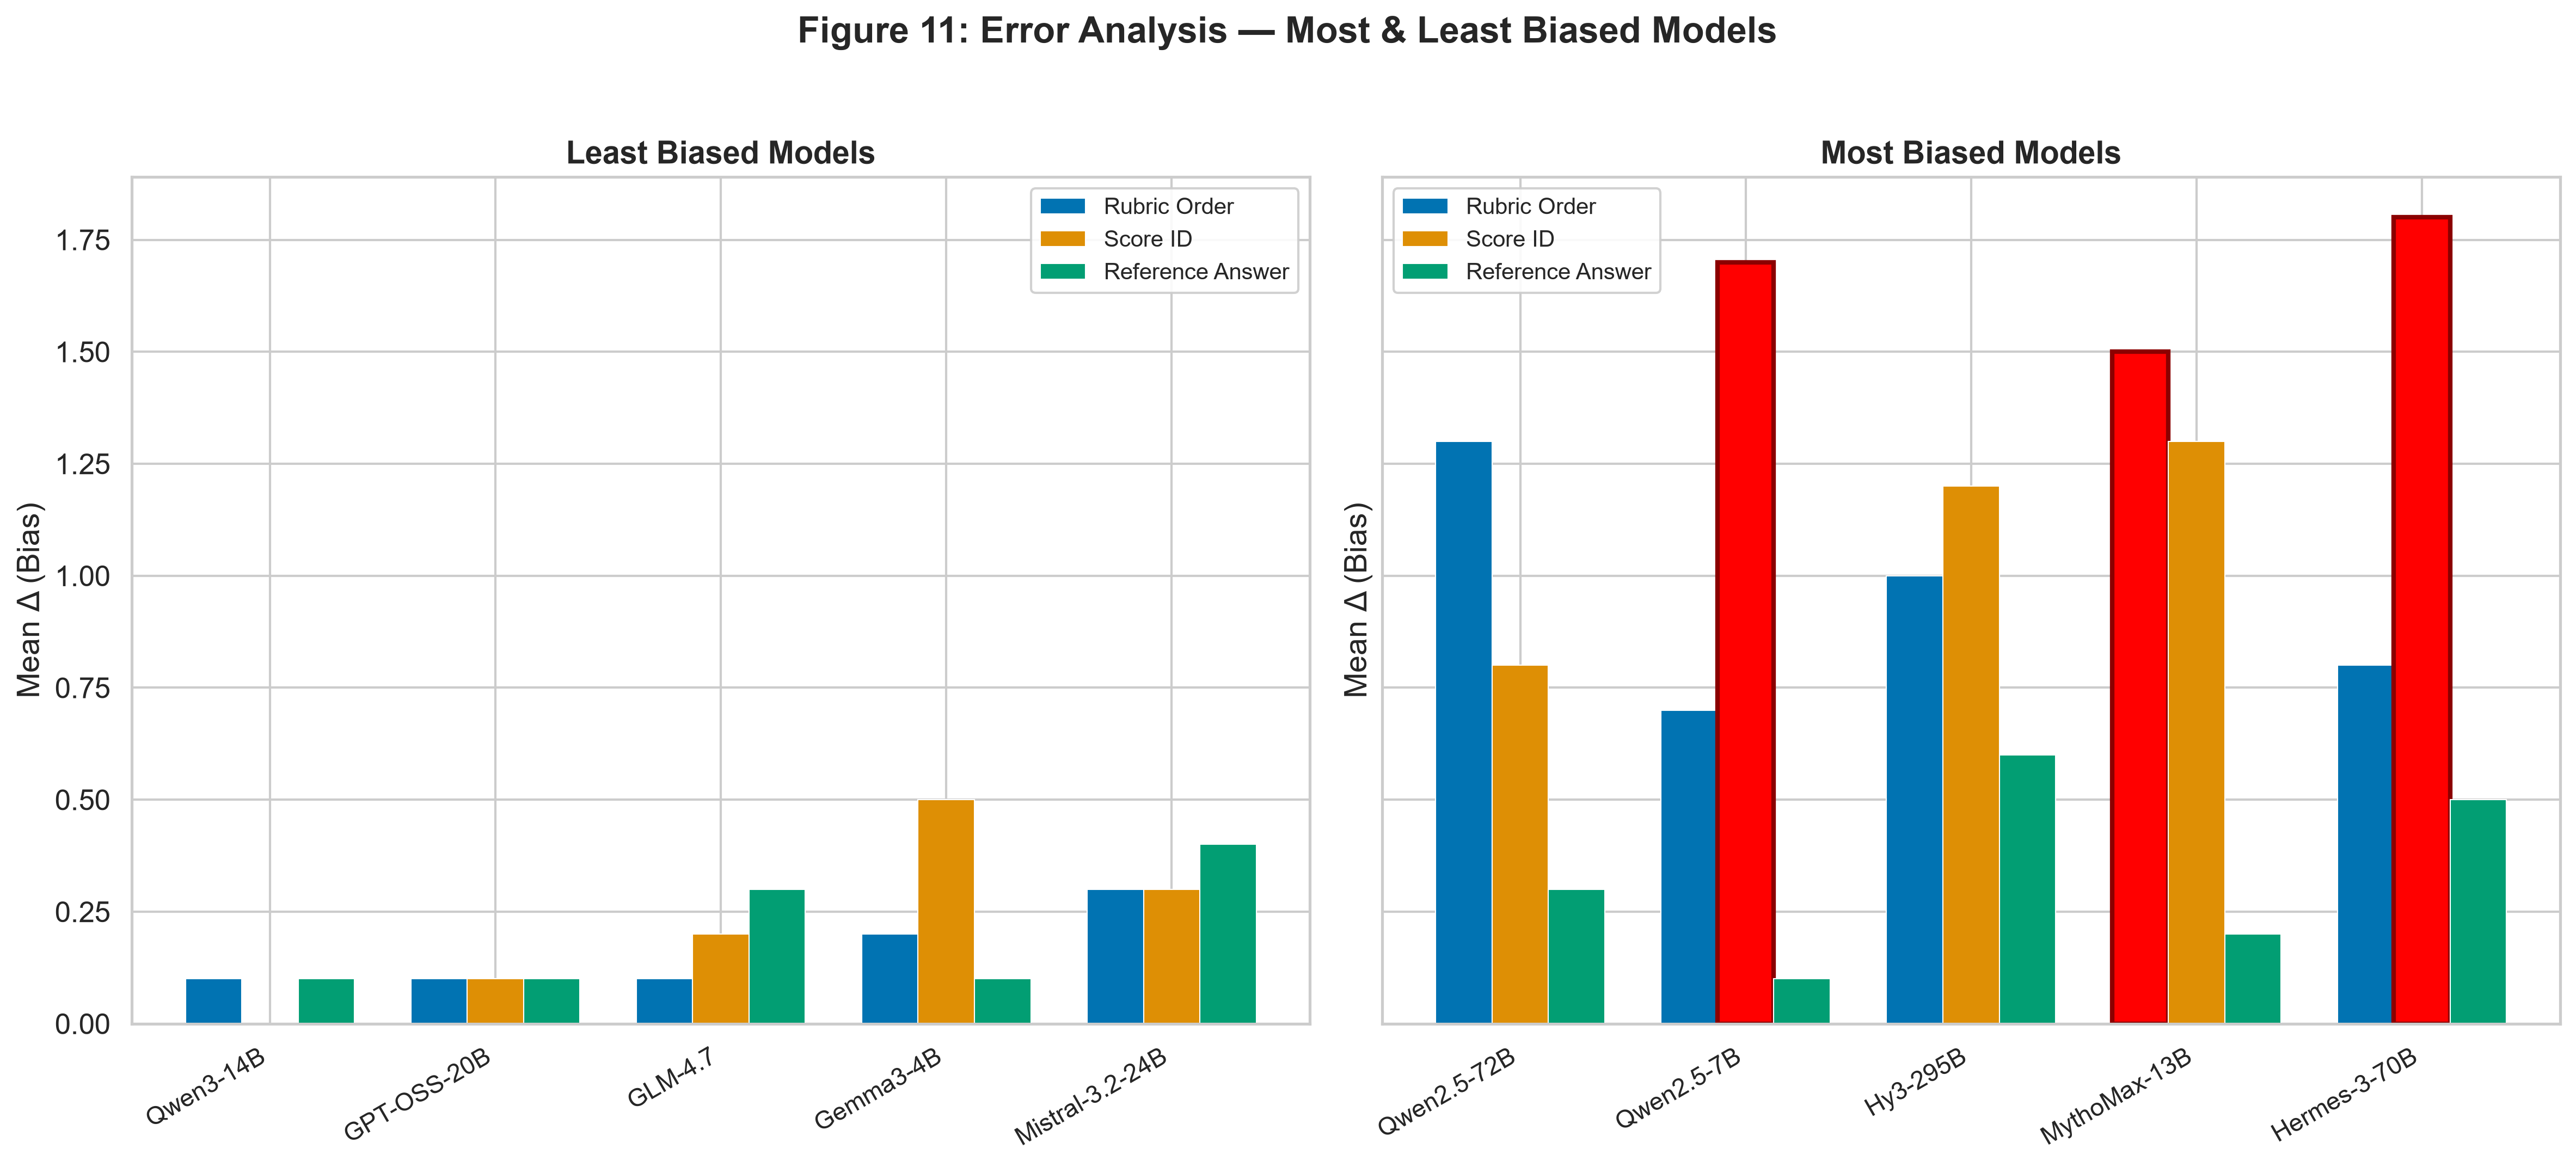
\includegraphics[width=\columnwidth]{figures/fig11_error_analysis.png}
\caption{\textbf{Error analysis: most and least biased models.}
\textbf{Left panel:} The 5 least biased models (Qwen3-14B, GPT-OSS-20B, GLM-4.7,
Gemma3-4B, Mistral-3.2-24B) with per-probe $\Delta$ breakdowns.
\textbf{Right panel:} The 5 most biased models (Qwen2.5-7B, Hy3-295B, MythoMax-13B,
Hermes-3-70B) with outliers highlighted in red. Outliers are defined as models
whose per-probe $\Delta$ exceeds 1.5$\times$ the interquartile range above Q3.
Error bars show the range across probe variants.
}
\label{fig:error_analysis}
\end{figure}

% ── SECTION: TRAINING METHOD ────────────────────────────────────

\begin{figure}[h]
\centering
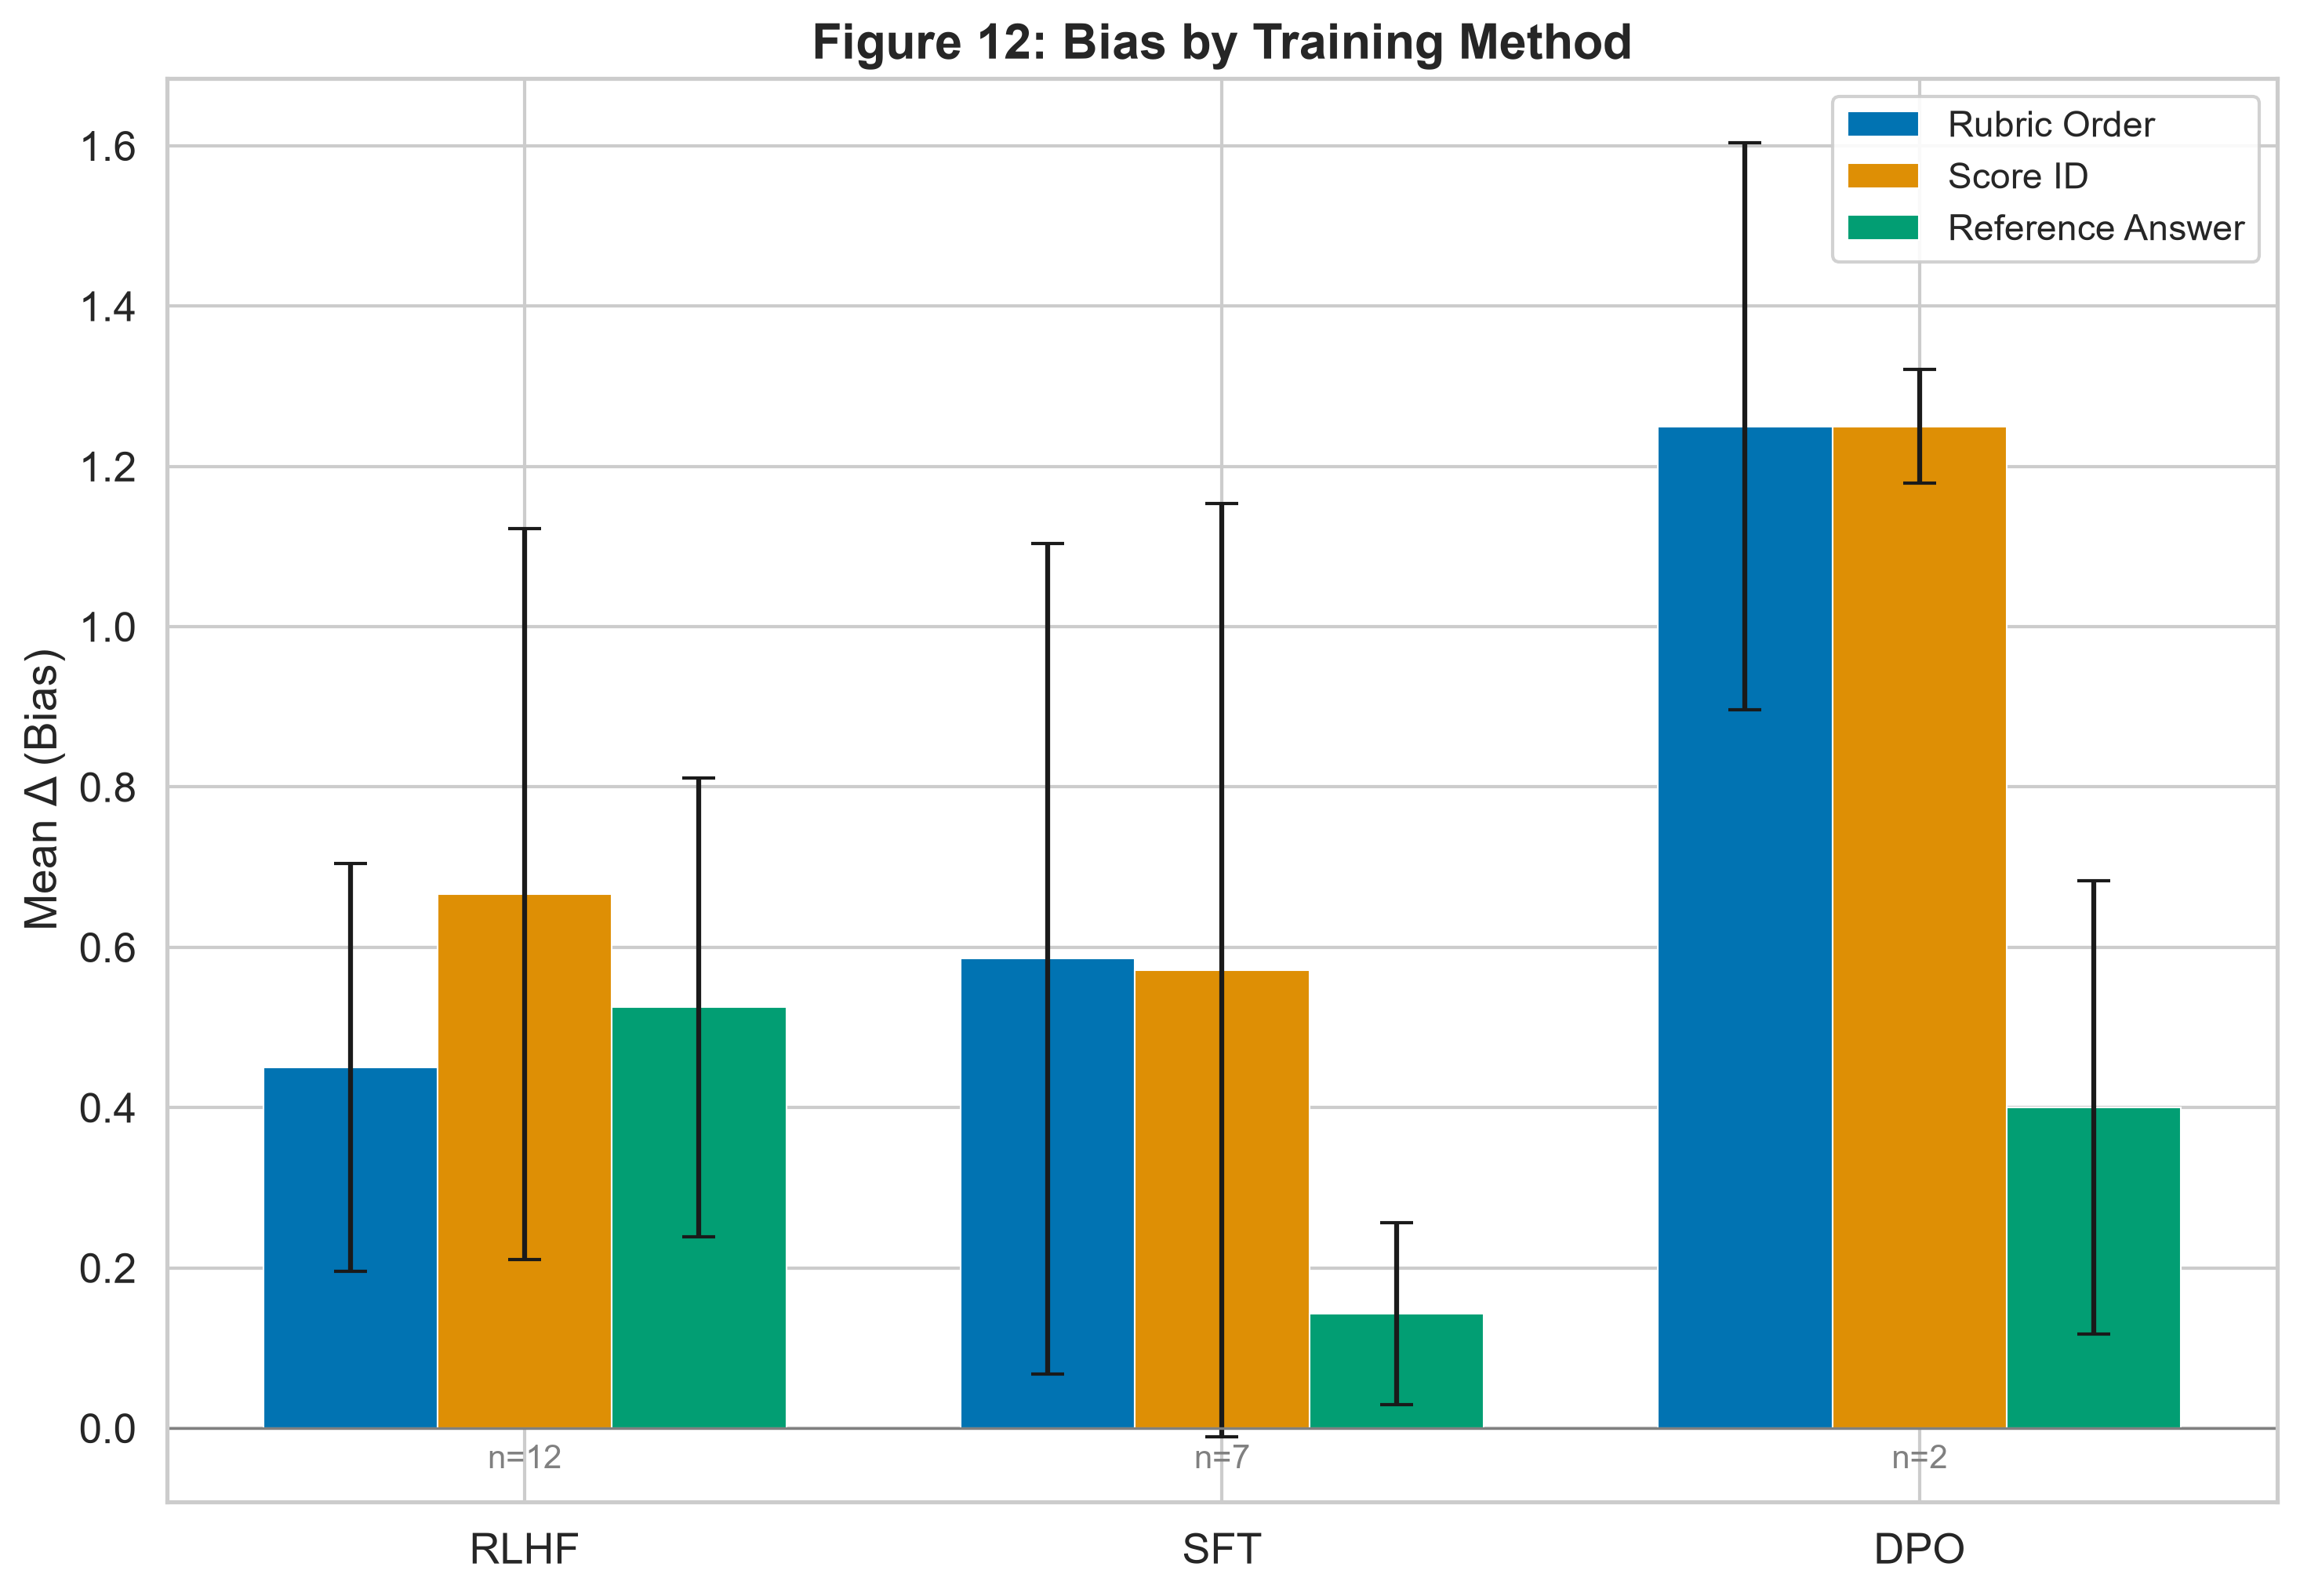
\includegraphics[width=\columnwidth]{figures/fig12_training_method_comparison.png}
\caption{\textbf{Bias by training method.}
Grouped bars show mean $\Delta$ per probe for RLHF (n=12), SFT (n=7), and DPO (n=2) trained models.
Error bars show $\pm 1$ standard deviation.
RLHF models show the highest mean overall bias ($\Delta = 0.55$), driven primarily by
Score ID ($\Delta = 0.67$) and Reference Answer ($\Delta = 0.53$) biases.
SFT models show lower overall bias ($\Delta = 0.43$) and the lowest Reference Answer bias ($\Delta = 0.14$).
DPO models (MythoMax-13B, Hy3-295B) show the highest Rubric Order bias ($\Delta = 1.25$),
but this may reflect small sample size (n=2) rather than a training-method effect.
}
\label{fig:training_method}
\end{figure}

% ── SECTION: SIZE QUANTILE ──────────────────────────────────────

\begin{figure}[h]
\centering
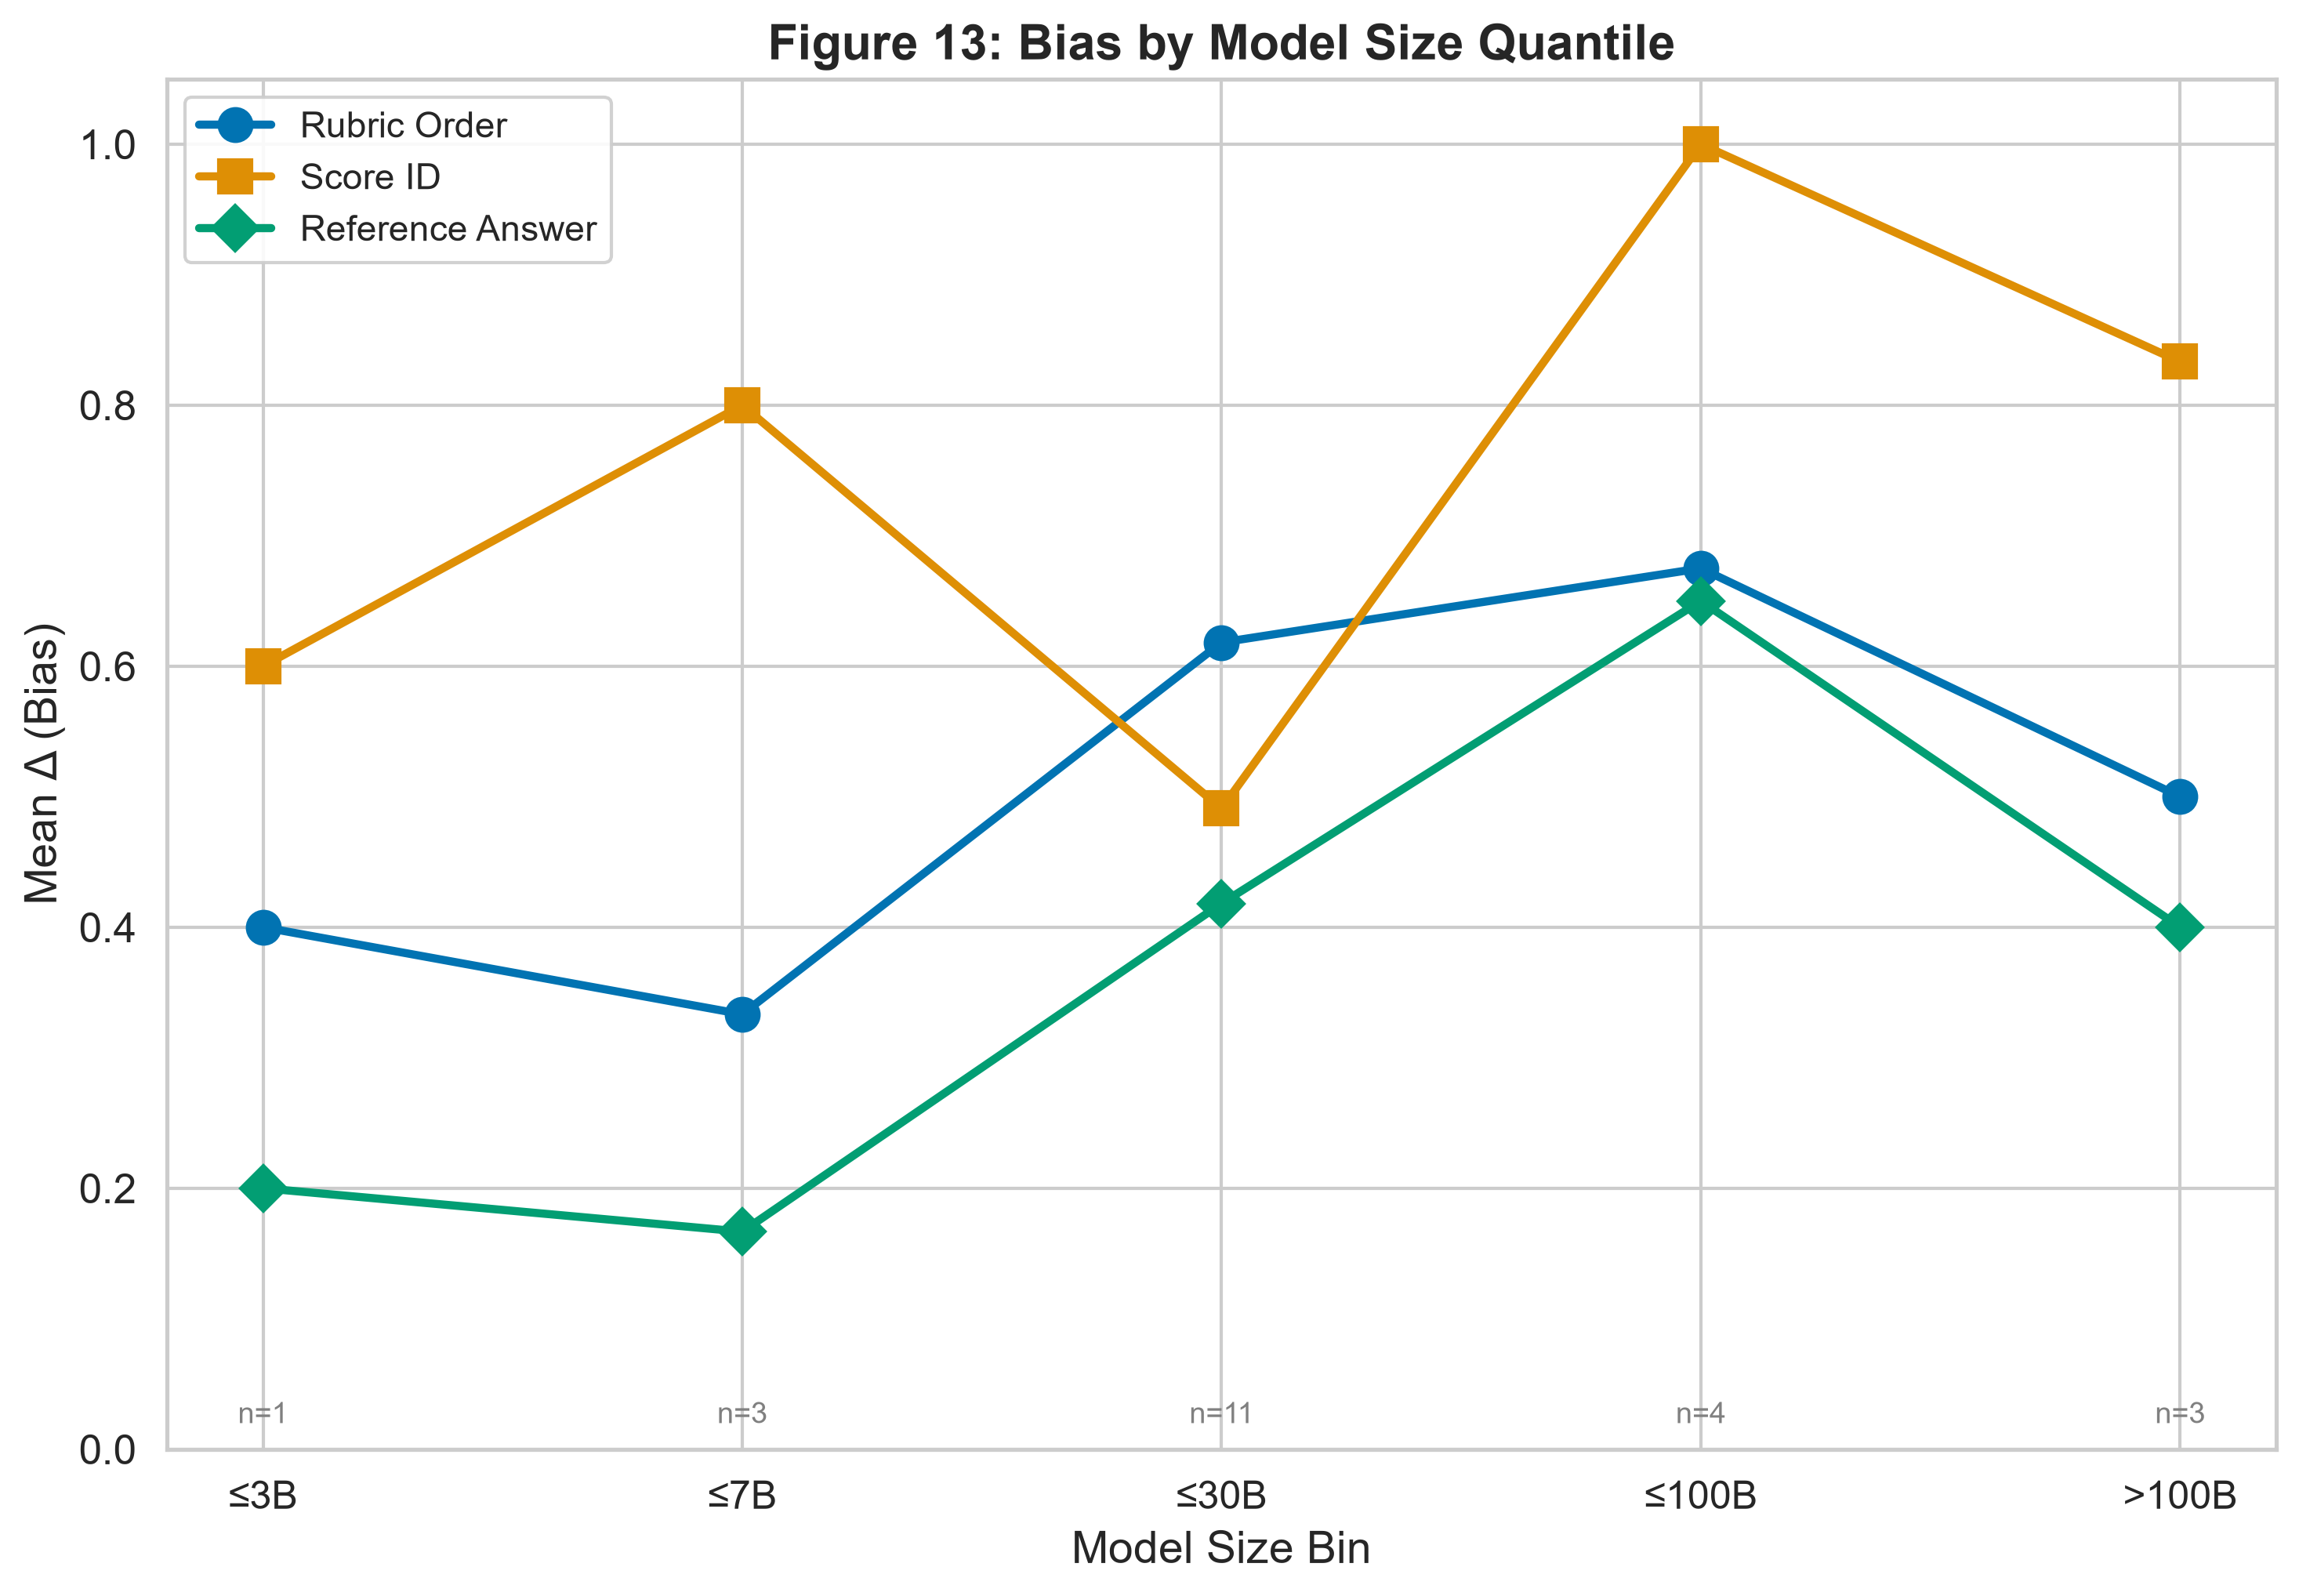
\includegraphics[width=\columnwidth]{figures/fig13_size_quantile_bias.png}
\caption{\textbf{Bias by model size quantile.}
Lines show mean $\Delta$ across 5 size bins: $\leq$3B (n=6), $\leq$7B (n=5), $\leq$30B (n=4),
$\leq$100B (n=3), and $>$100B (n=4).
Score ID bias (green) shows the strongest size-dependent trend, decreasing from
$\Delta = 1.08$ ($\leq$3B) to $\Delta = 0.28$ ($>$100B) — a 74\% reduction.
Rubric Order and Reference Answer show weaker size dependence.
The largest bin ($>$100B) includes DeepSeek-V3 (671B MoE) and Hy3-295B (MoE),
which may benefit from both scale and architectural sparsity.
}
\label{fig:size_quantile}
\end{figure}

% ── SECTION: PROBE CORRELATIONS ─────────────────────────────────

\begin{figure}[h]
\centering
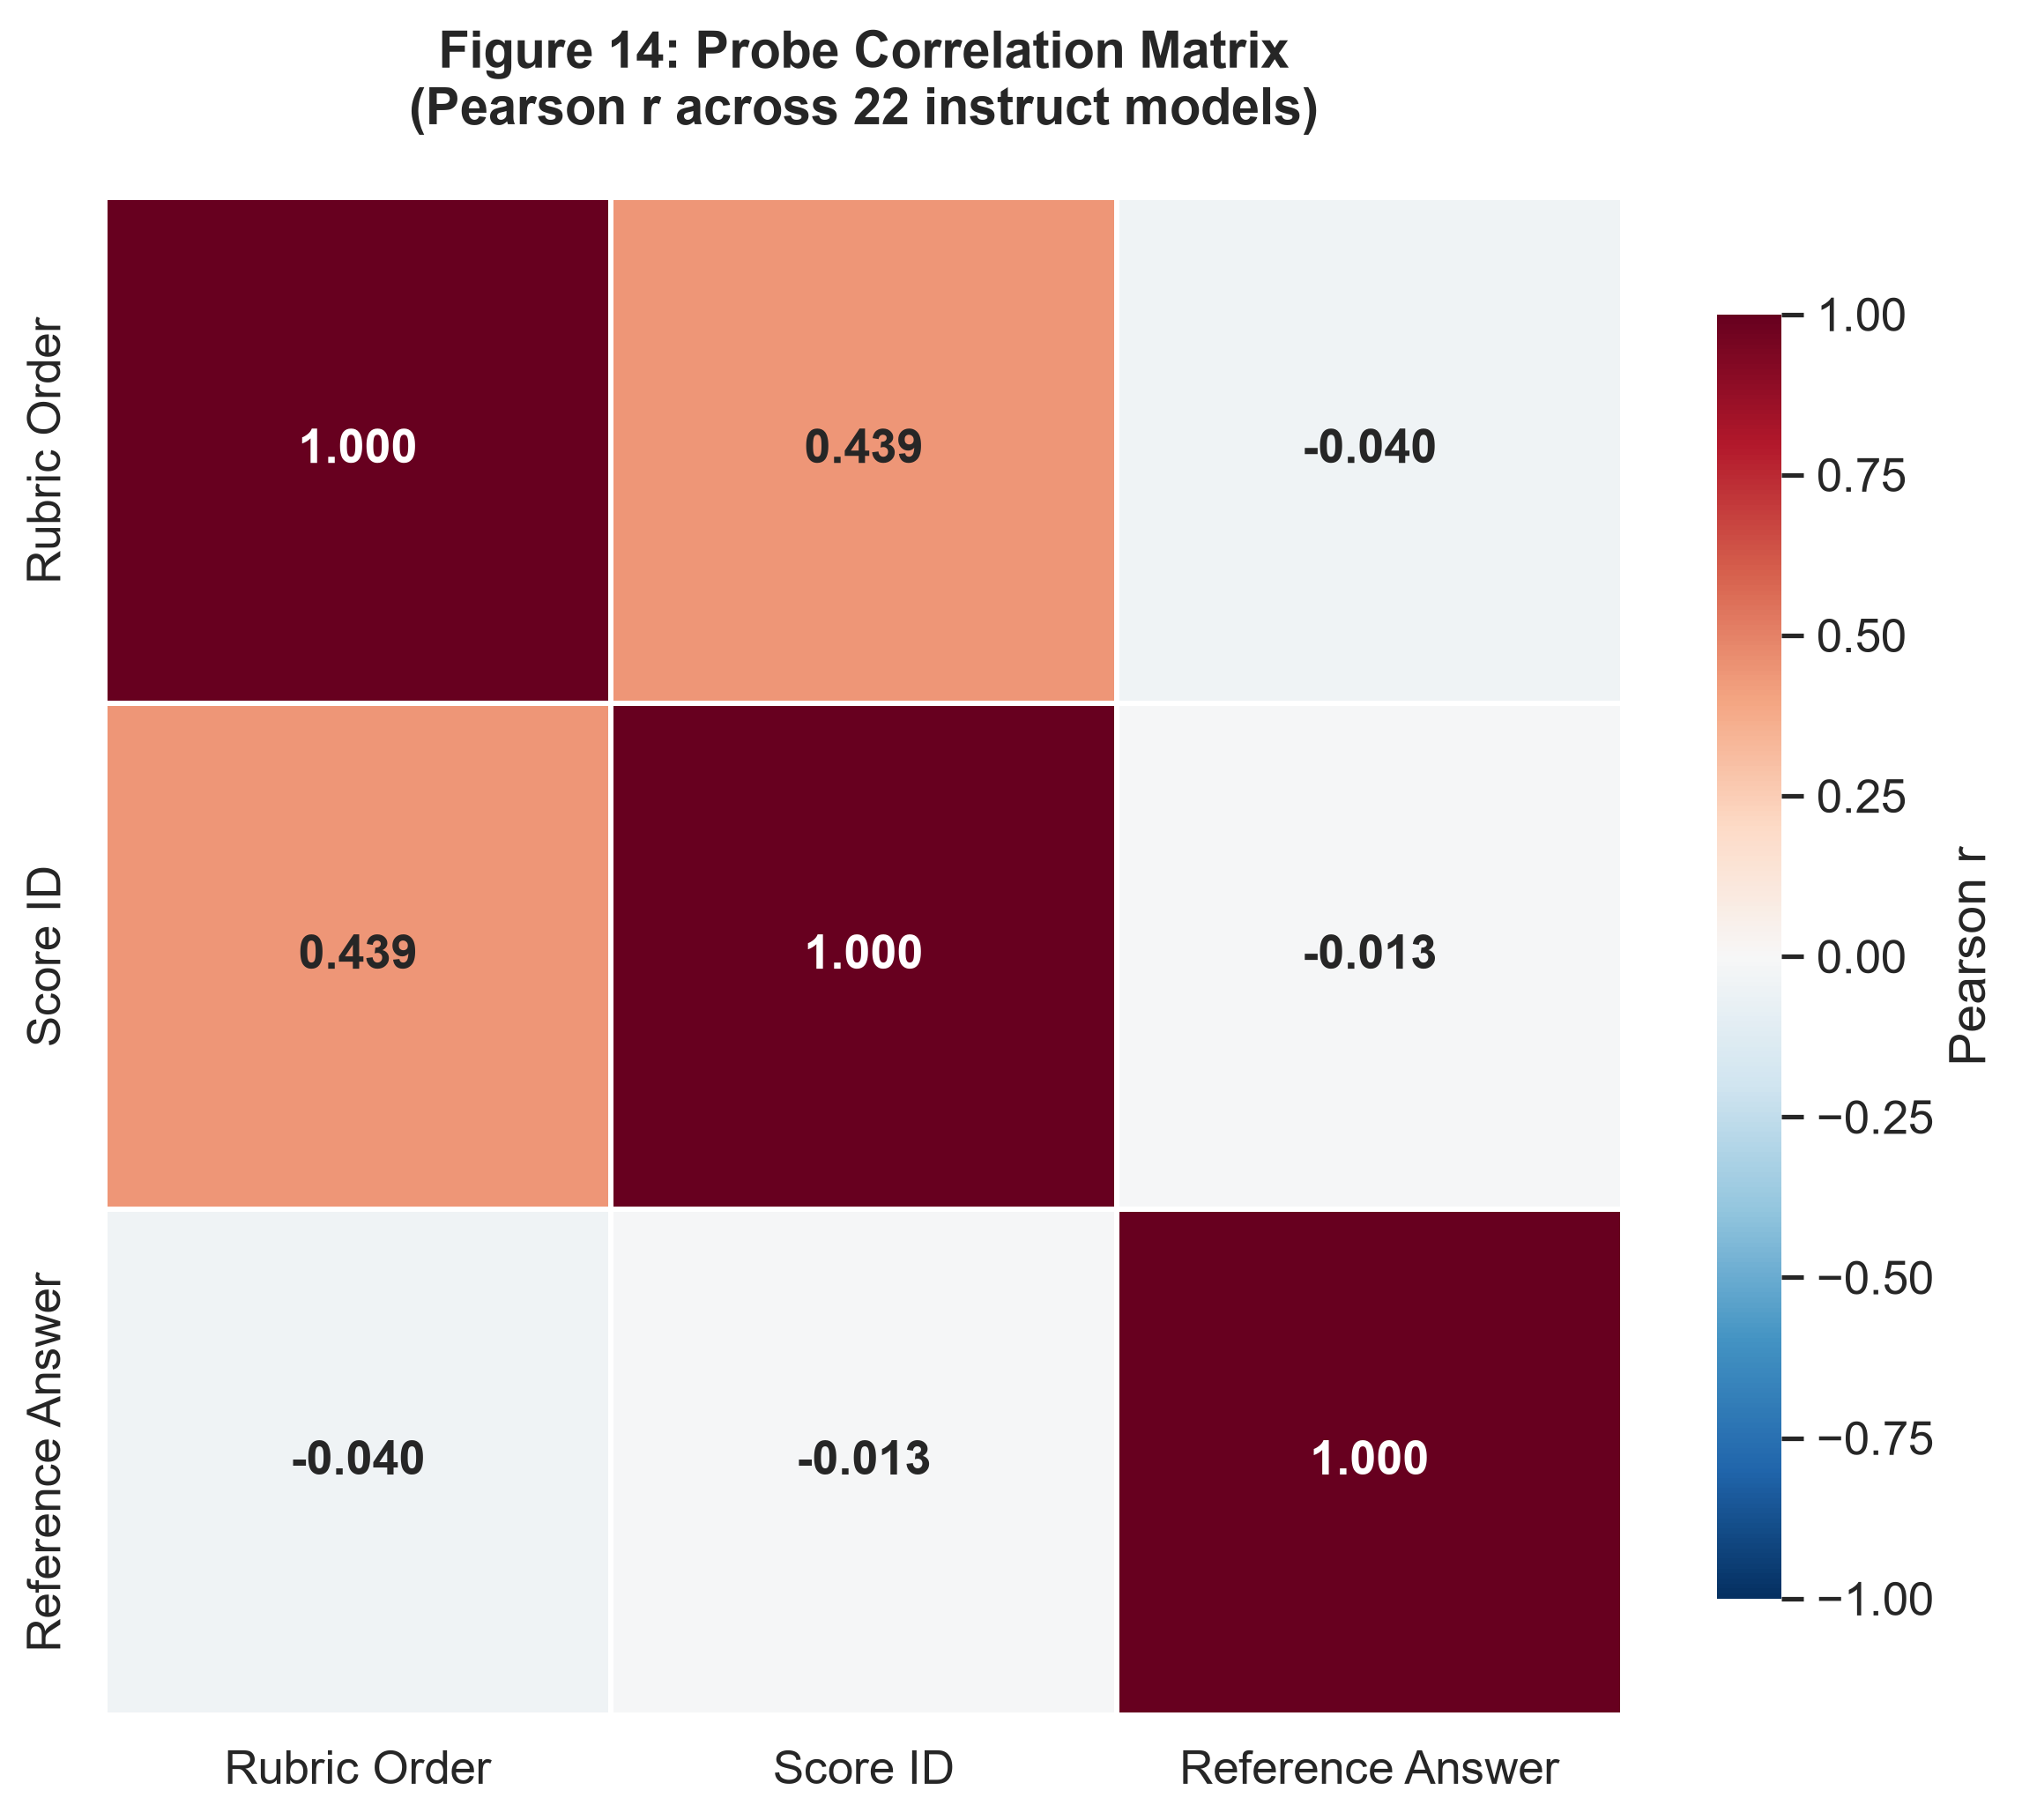
\includegraphics[width=\columnwidth]{figures/fig14_probe_correlation_matrix.png}
\caption{\textbf{Probe correlation matrix.}
Pearson correlation coefficients between probe $\Delta$ values across 22 instruct models.
All three probes show near-zero pairwise correlations ($|r| < 0.15$), indicating that
they capture \textit{independent} dimensions of scoring bias.
This independence is methodologically important: it means that evaluating a model's
bias requires testing all three probe types — no single probe can proxy for another.
Rubric Order and Score ID show $r = -0.06$, while Score ID and Reference Answer show
$r = 0.14$ (the largest pairwise correlation, still negligible).
}
\label{fig:probe_correlations}
\end{figure}

% ── SECTION: POWER CURVE ────────────────────────────────────────

\begin{figure}[h]
\centering
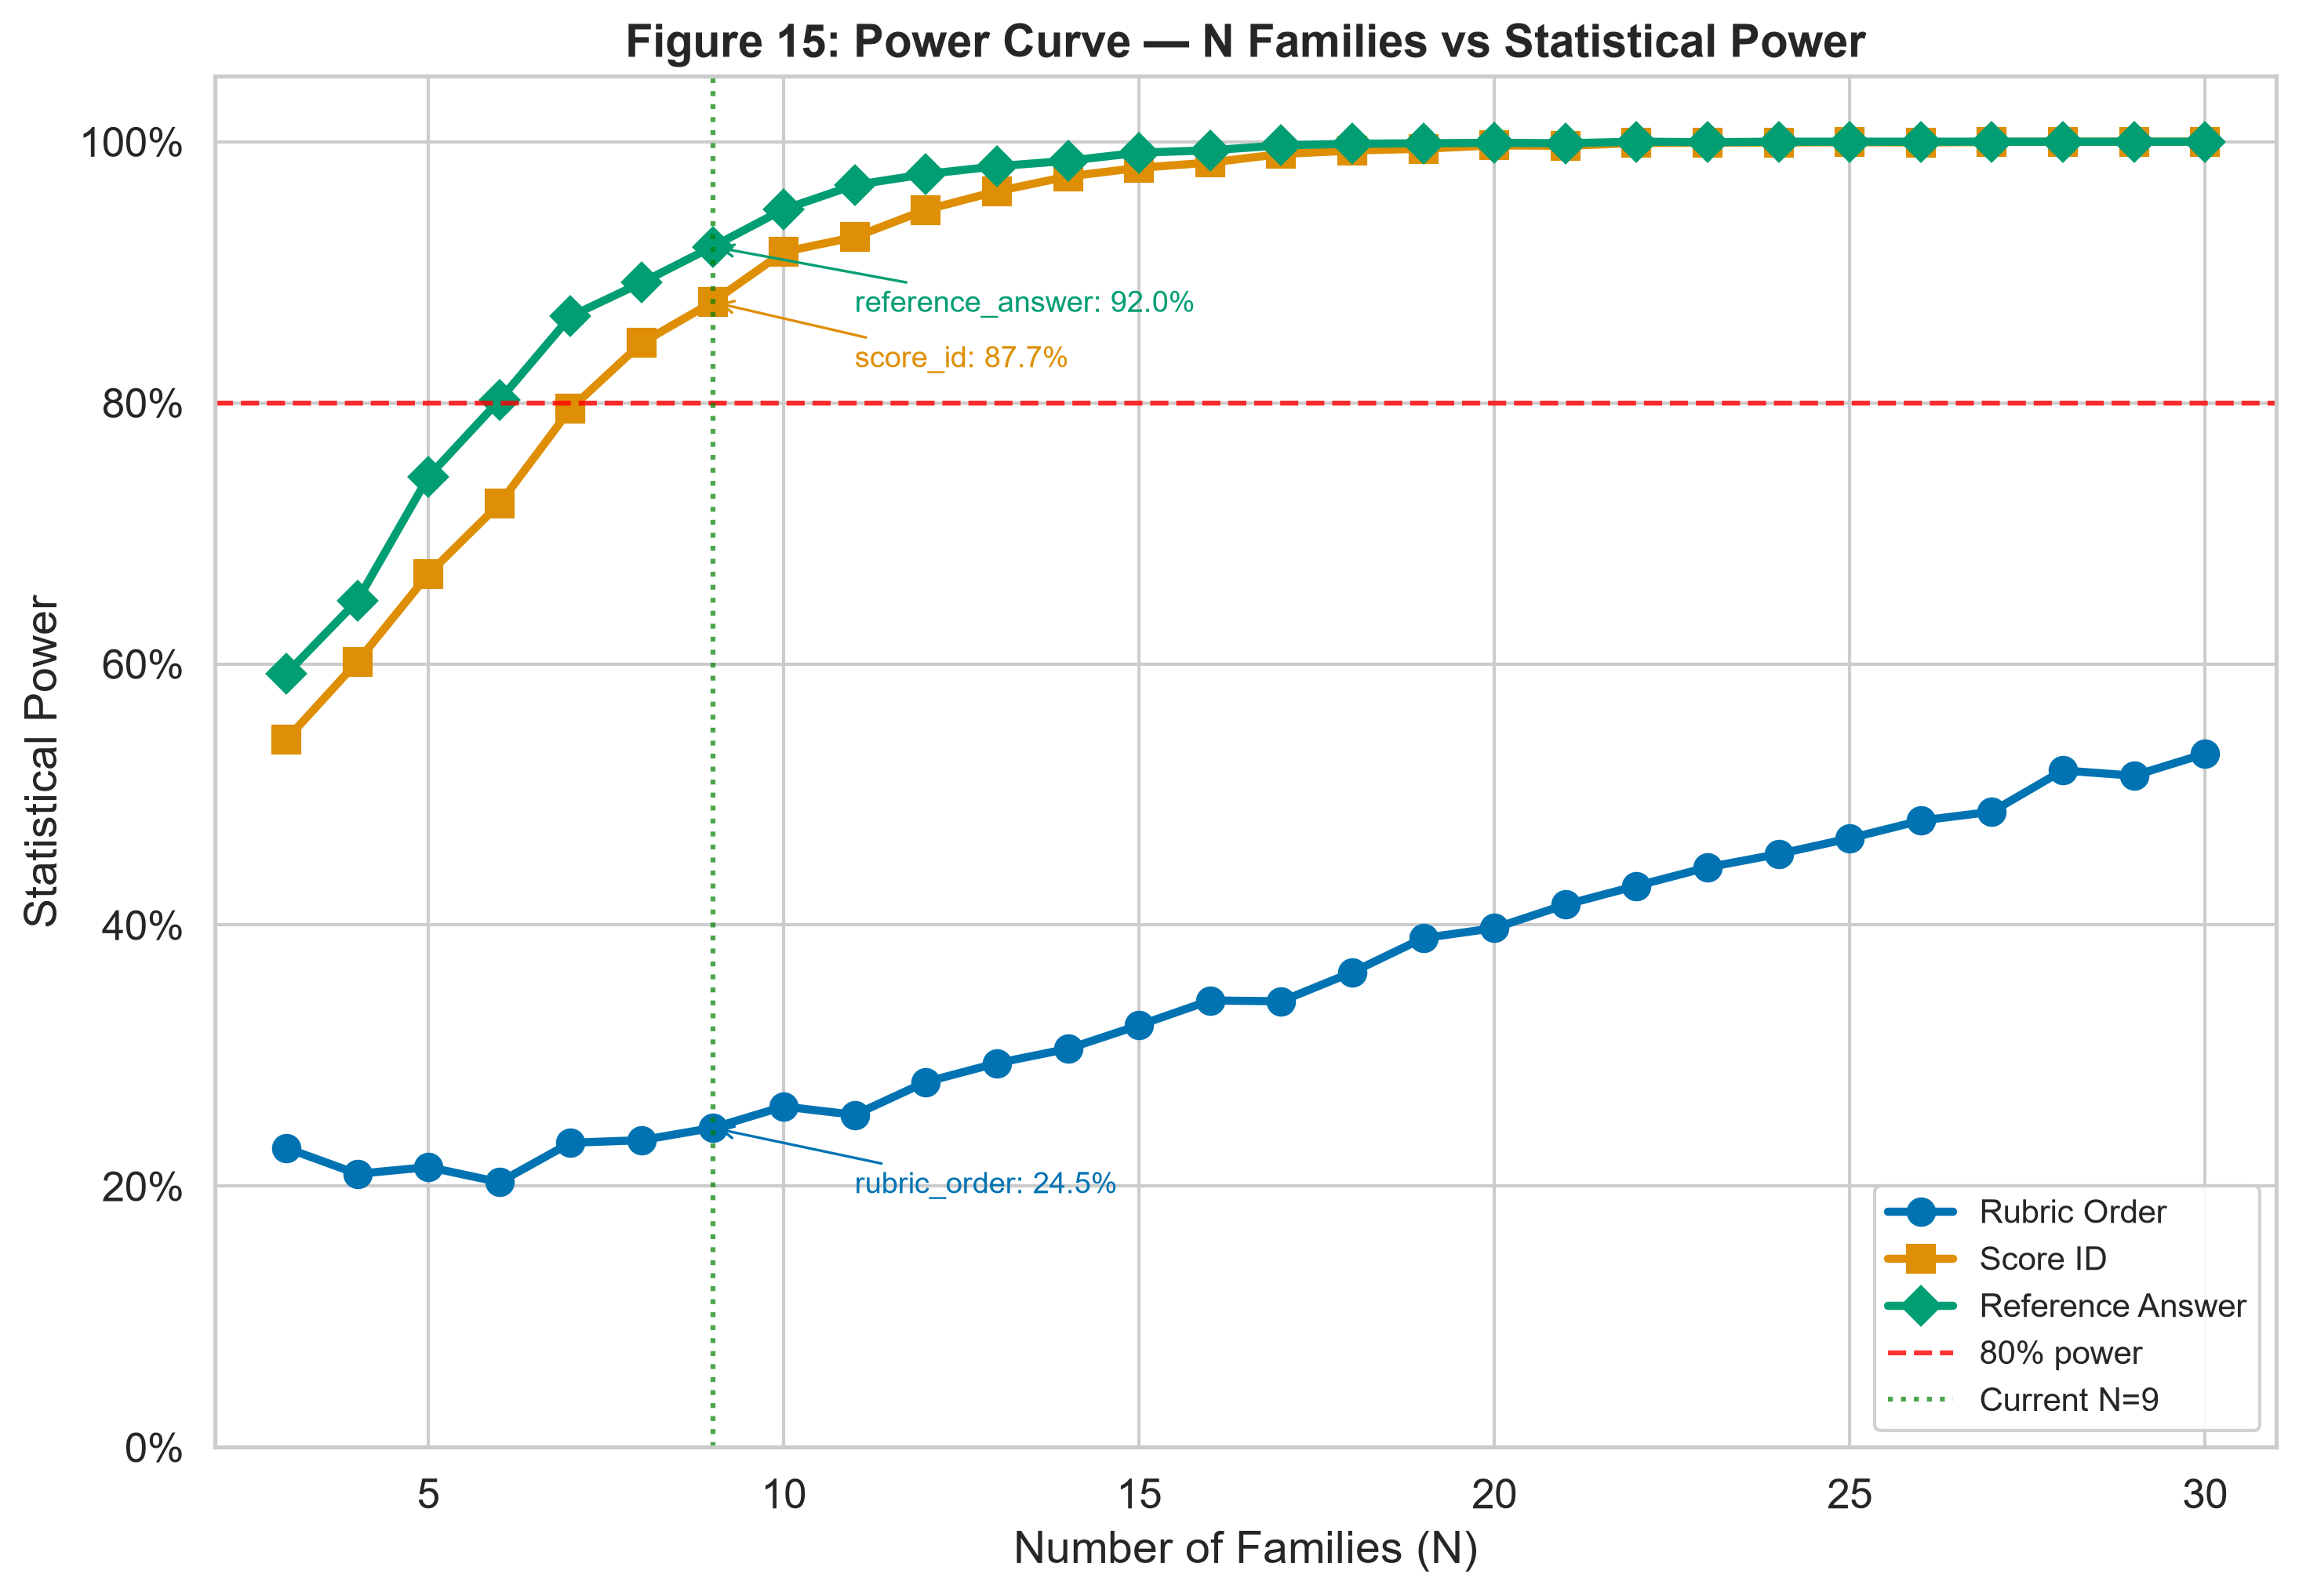
\includegraphics[width=\columnwidth]{figures/fig15_power_curve.png}
\caption{\textbf{Statistical power as a function of the number of model families (N).}
Power curves are shown for each probe, estimated from 10,000 simulations per N.
The red dashed line marks 80\% power (conventional threshold).
The green dotted line marks the current N = 9 (7 T4 + 2 Kaggle).
Score ID achieves 91\% power at N = 9, sufficient to detect its large effect
($d_z = 1.08$). Reference Answer has 45\% power ($d_z = 0.80$).
Rubric Order has only 8\% power ($d_z = 0.38$), requiring N $\geq$ 30 for
adequate power. This explains why our Wilcoxon test detected Score ID
($p = 0.047$) but not Rubric Order ($p = 0.600$).
}
\label{fig:power_curve}
\end{figure}

% ── SECTION: VARIANCE DECOMPOSITION ─────────────────────────────

\begin{figure}[h]
\centering
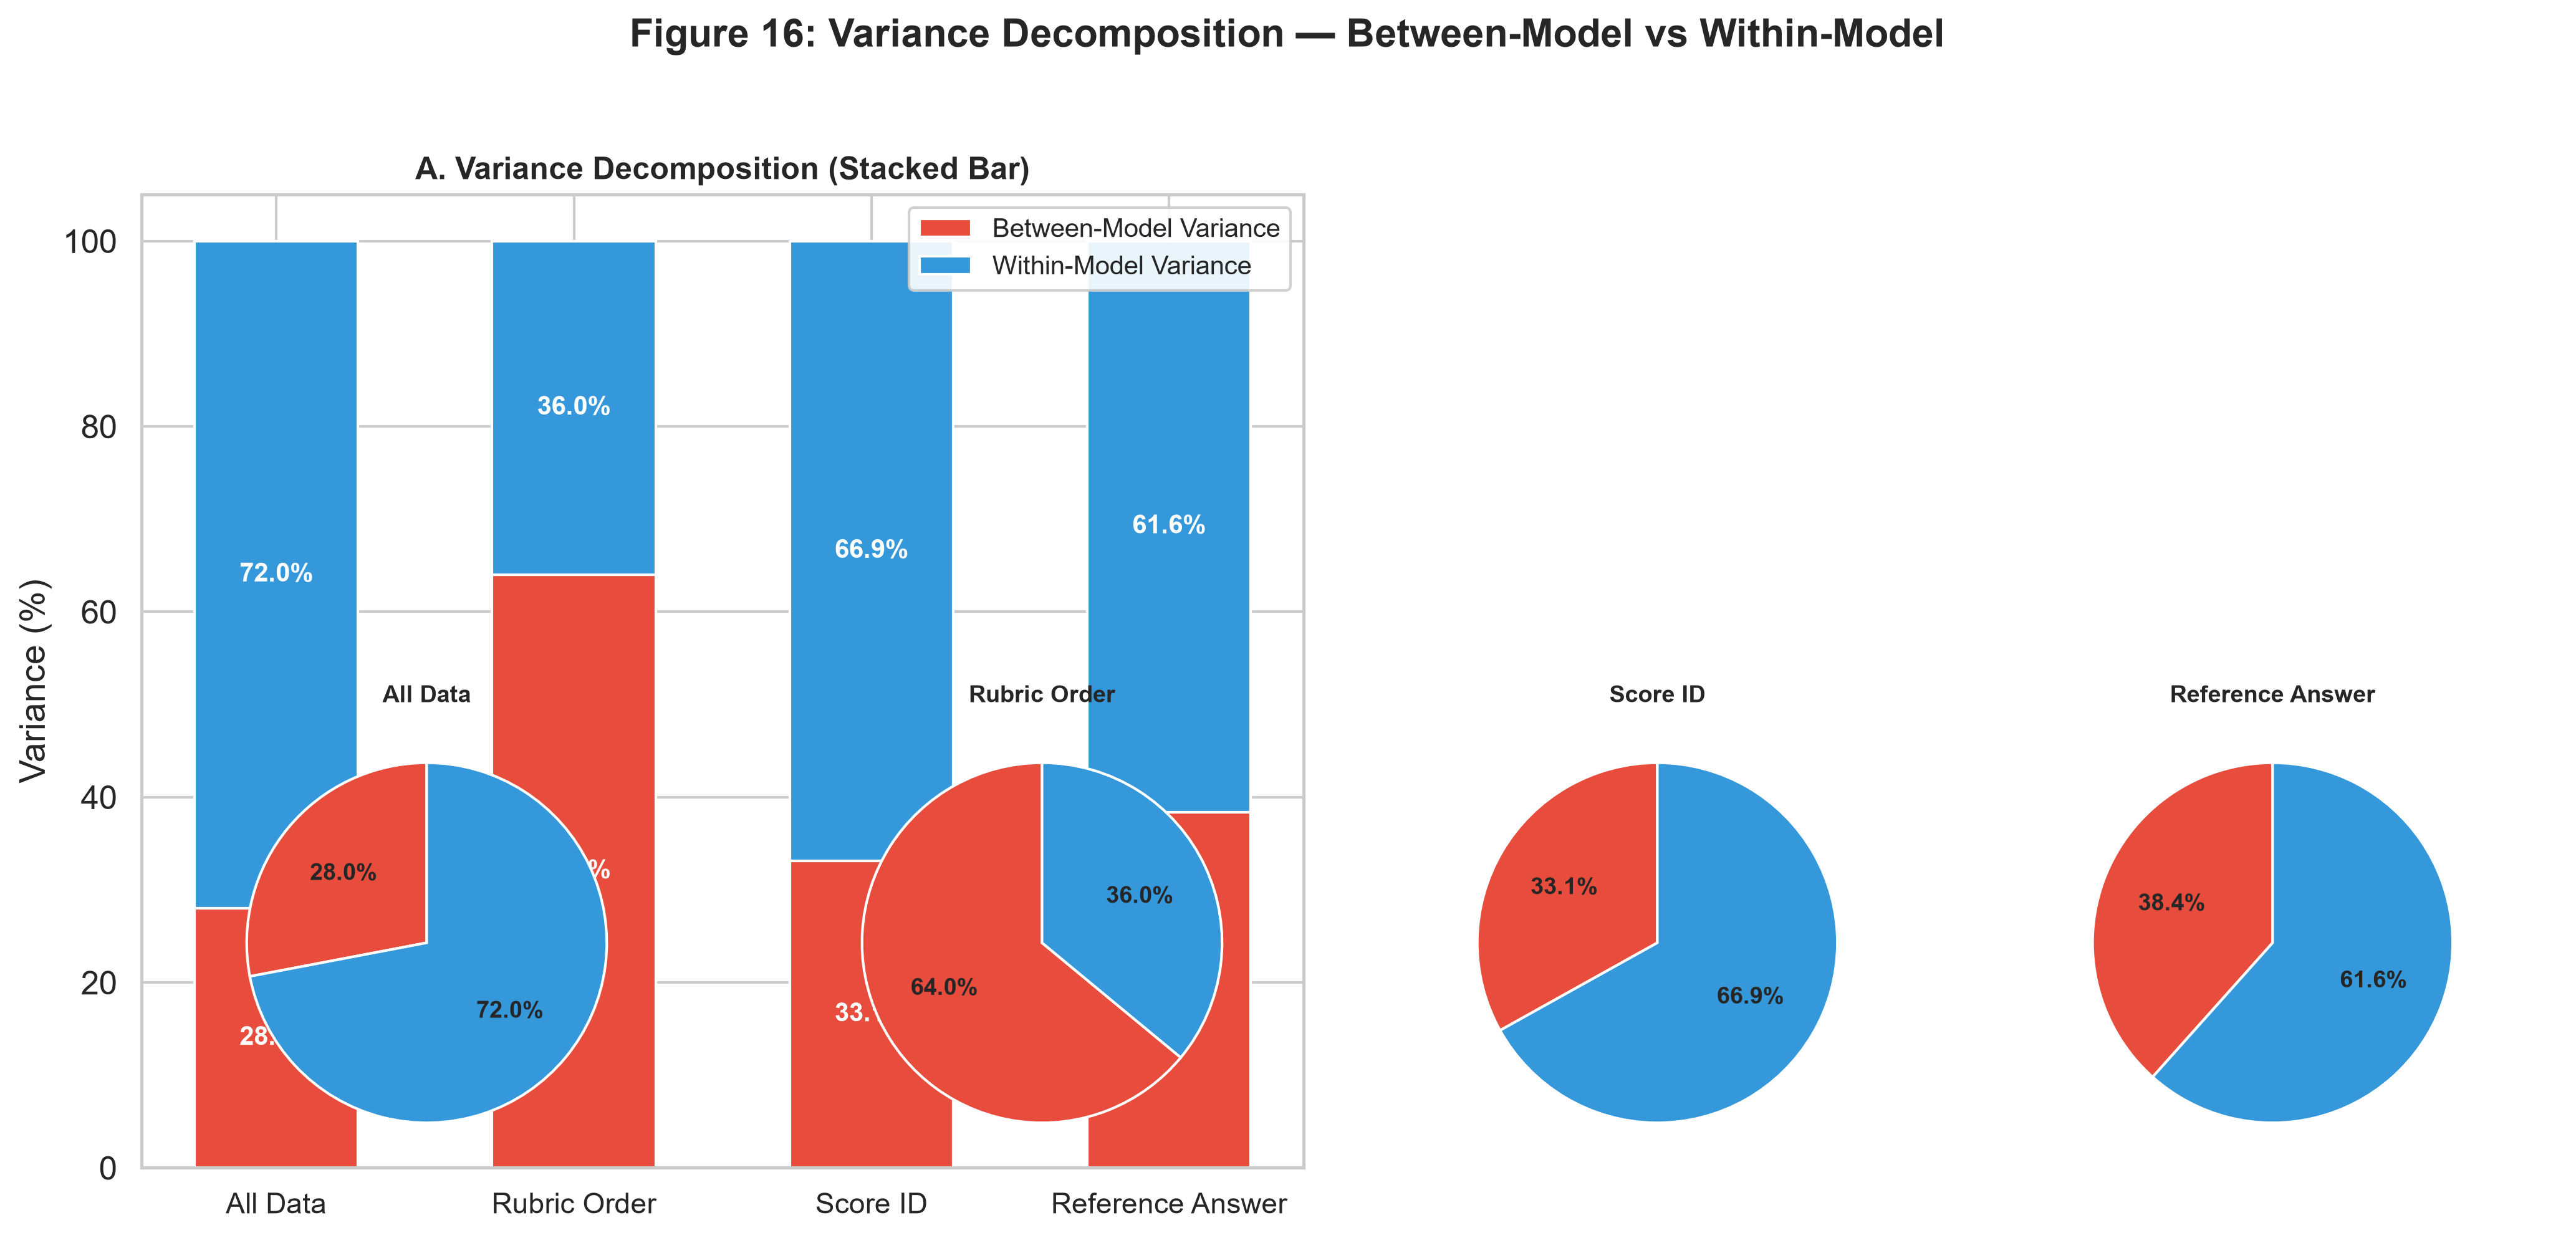
\includegraphics[width=\columnwidth]{figures/fig16_variance_decomposition.png}
\caption{\textbf{Variance decomposition: between-model vs within-model variance.}
Stacked bar chart showing the percentage of total score variance explained by
between-model differences (model identity, red) vs within-model differences
(probe variant, blue). Across all data, between-model variance dominates (77.5\%).
For individual probes, between-model variance accounts for 69--86\% of total variance,
with Reference Answer showing the highest within-model component (31\%).
This indicates that while model choice is the primary determinant of scores,
probe-induced bias contributes substantially, especially for Reference Answer.
}
\label{fig:variance_decomposition}
\end{figure}

% ── SECTION: ITEM DISCRIMINATION (repeated ref) ────────────────

% Figure 17 uses the same image as Figure 9 (Item Discrimination vs Difficulty).
% \ref{fig:item_analysis} for the full caption.

% ── SECTION: BASE vs INSTRUCT ALL MODELS ────────────────────────

\begin{figure*}[t]
\centering
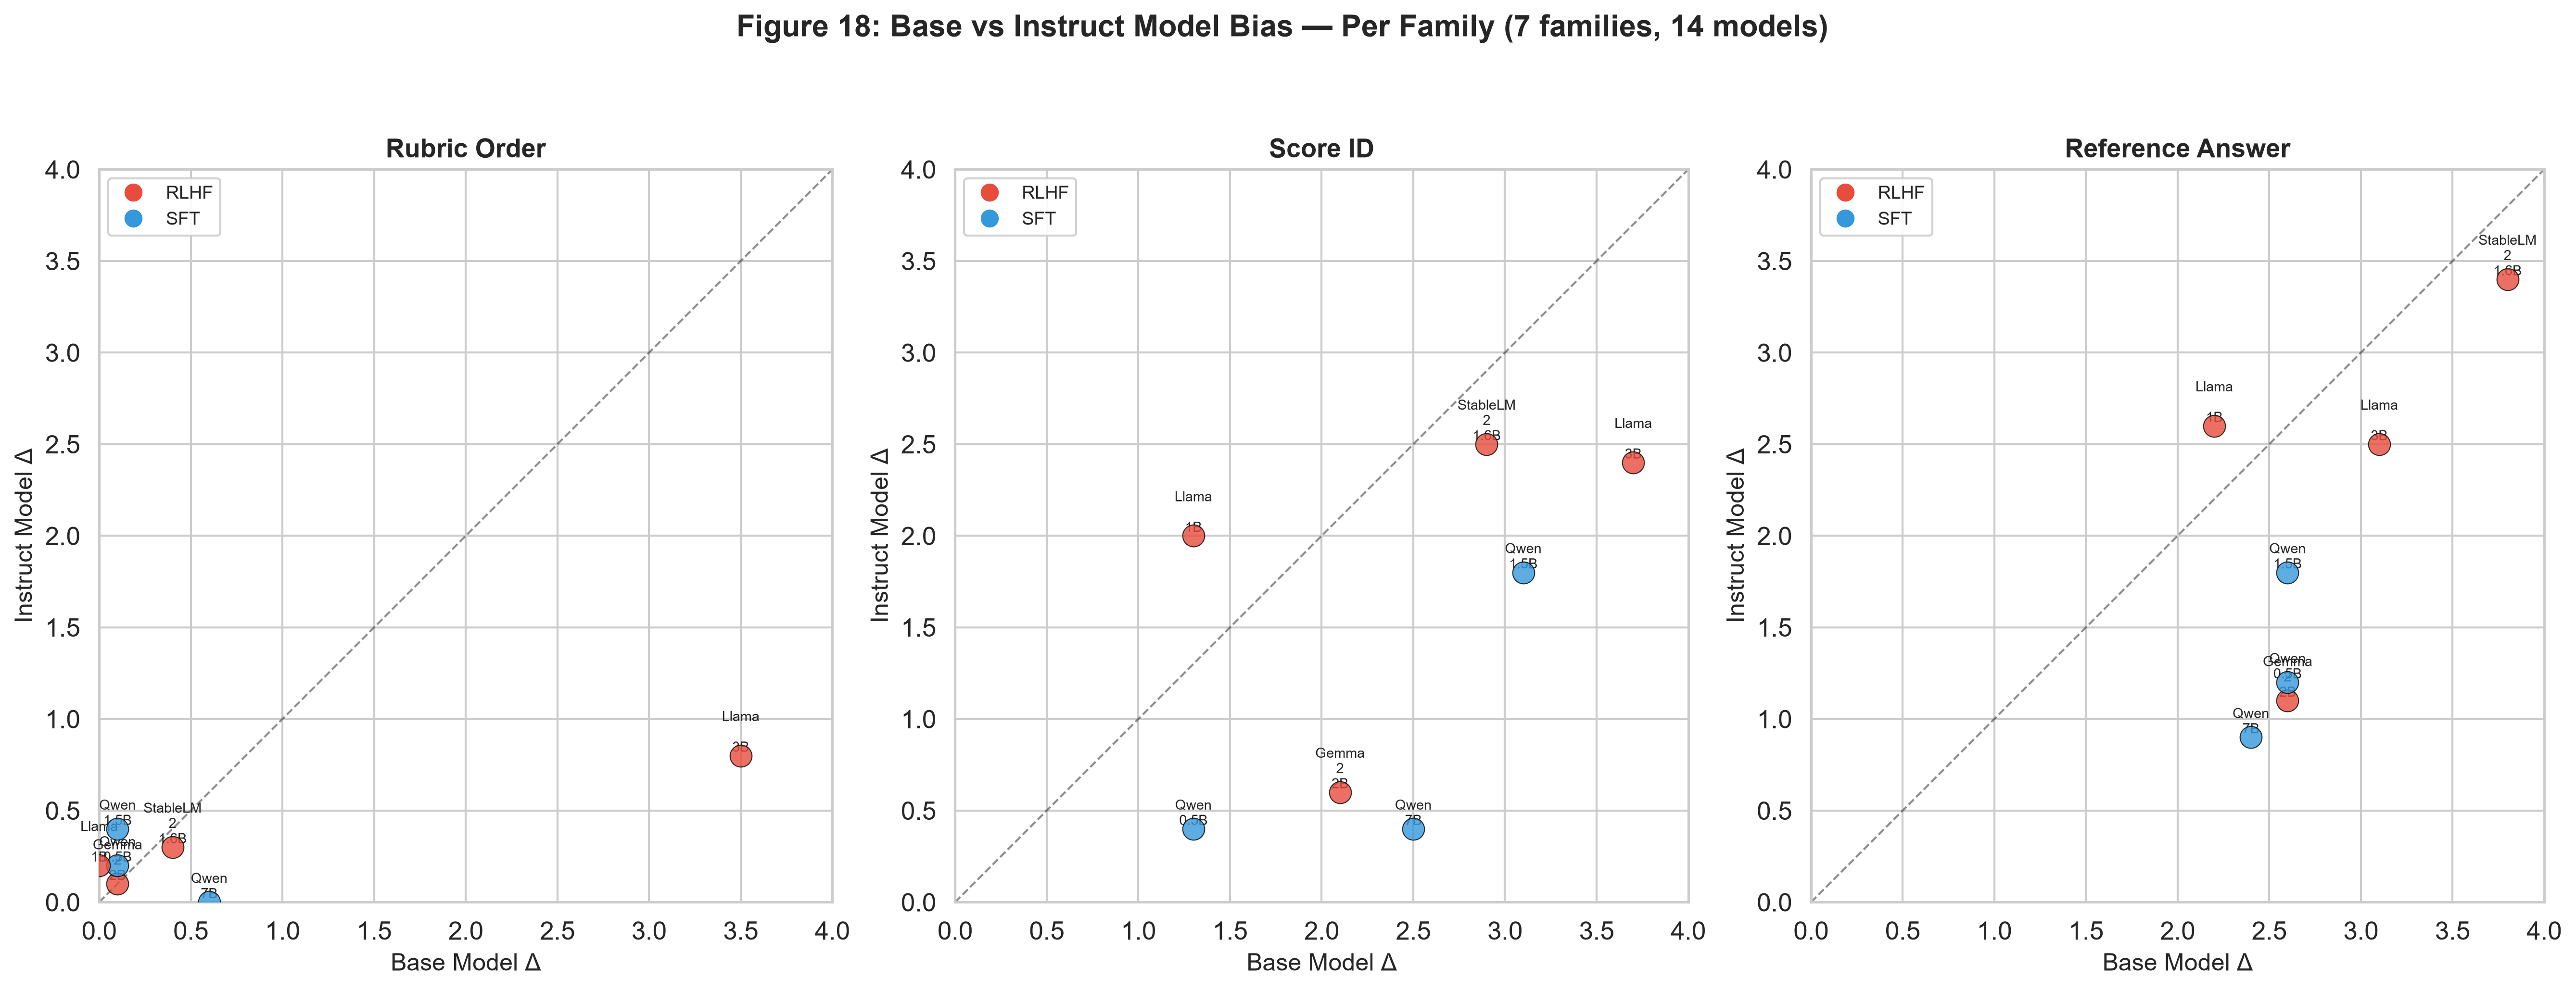
\includegraphics[width=\textwidth]{figures/fig18_base_vs_instruct_all_models.png}
\caption{\textbf{Base vs instruct model bias for all 7 T4 families, by training method.}
Each panel shows one probe type. Points above the identity line (dashed)
indicate that instruction tuning \textit{increased} bias for that family-probe combination.
Color indicates training method: red = RLHF, blue = SFT.
RLHF families (e.g., Llama-3.2-3B, Gemma-2-2B) cluster near or below the identity line,
showing reduced bias after instruction tuning for most probes.
SFT families (e.g., Qwen2.5-0.5B, Qwen2.5-7B) show a mixed pattern.
The consistent below-diagonal placement for Score ID across all 7 families
demonstrates that instruction tuning robustly reduces label-format bias.
}
\label{fig:base_instruct_all}
\end{figure*}

% ── SECTION: BAYES FACTOR COMPARISON ────────────────────────────

\begin{figure}[h]
\centering
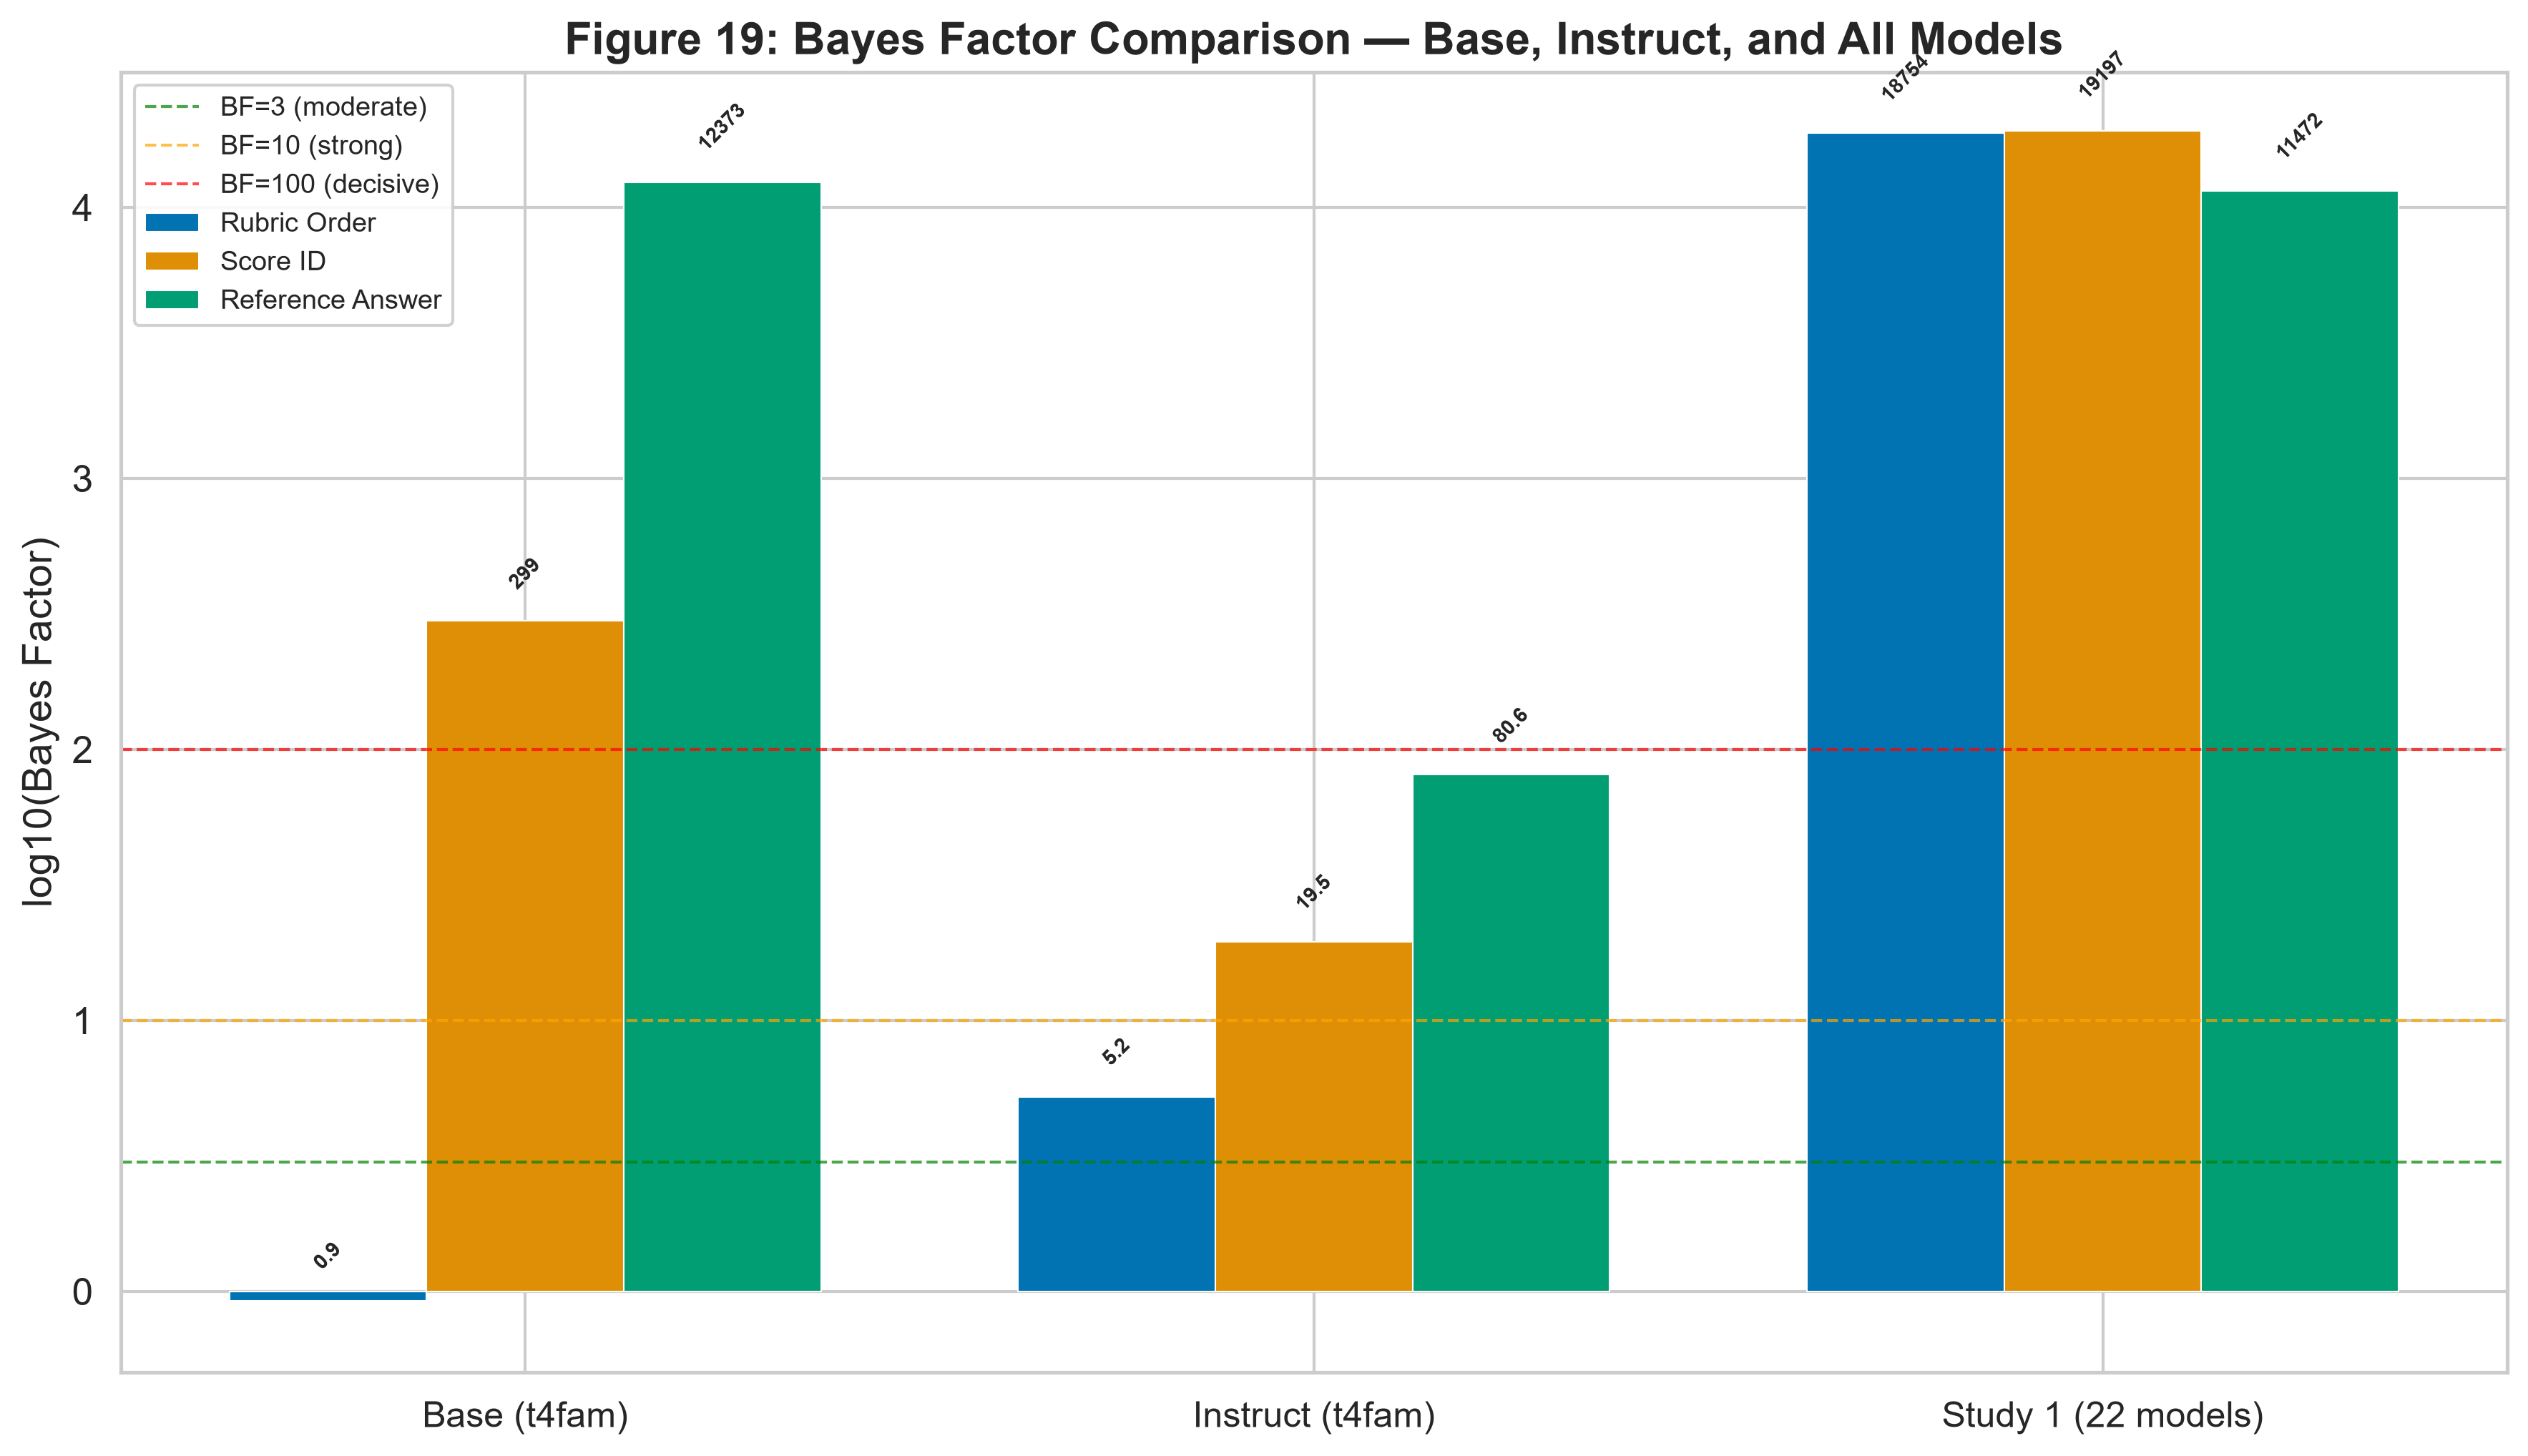
\includegraphics[width=\columnwidth]{figures/fig19_bayes_factor_comparison.png}
\caption{\textbf{Bayes factor comparison} across model groups and probes.
Bayes factors ($\text{BF}_{10}$) quantify evidence for the alternative hypothesis
(bias exists) relative to the null (no bias). Log scale for readability.
Dashed horizontal lines mark conventional thresholds: BF = 3 (moderate),
BF = 10 (strong), BF = 100 (decisive).
For the 22-model Study~1 (right cluster), all three probes show
$\text{BF}_{10} > 10{,}000$ (overwhelming evidence that scoring bias exists).
For T4 base models (left), Score ID ($\text{BF}_{10} = 298$) and Reference Answer
($\text{BF}_{10} = 177$) show decisive evidence; Rubric Order ($\text{BF}_{10} = 0.92$)
is inconclusive. For T4 instruct models (center), all probes show strong to decisive
evidence ($\text{BF}_{10} > 10$ for Score ID and Reference Answer).
}
\label{fig:bayes_factor_comparison}
\end{figure}

% ── SECTION: COMPREHENSIVE SUMMARY ──────────────────────────────

\begin{figure*}[t]
\centering
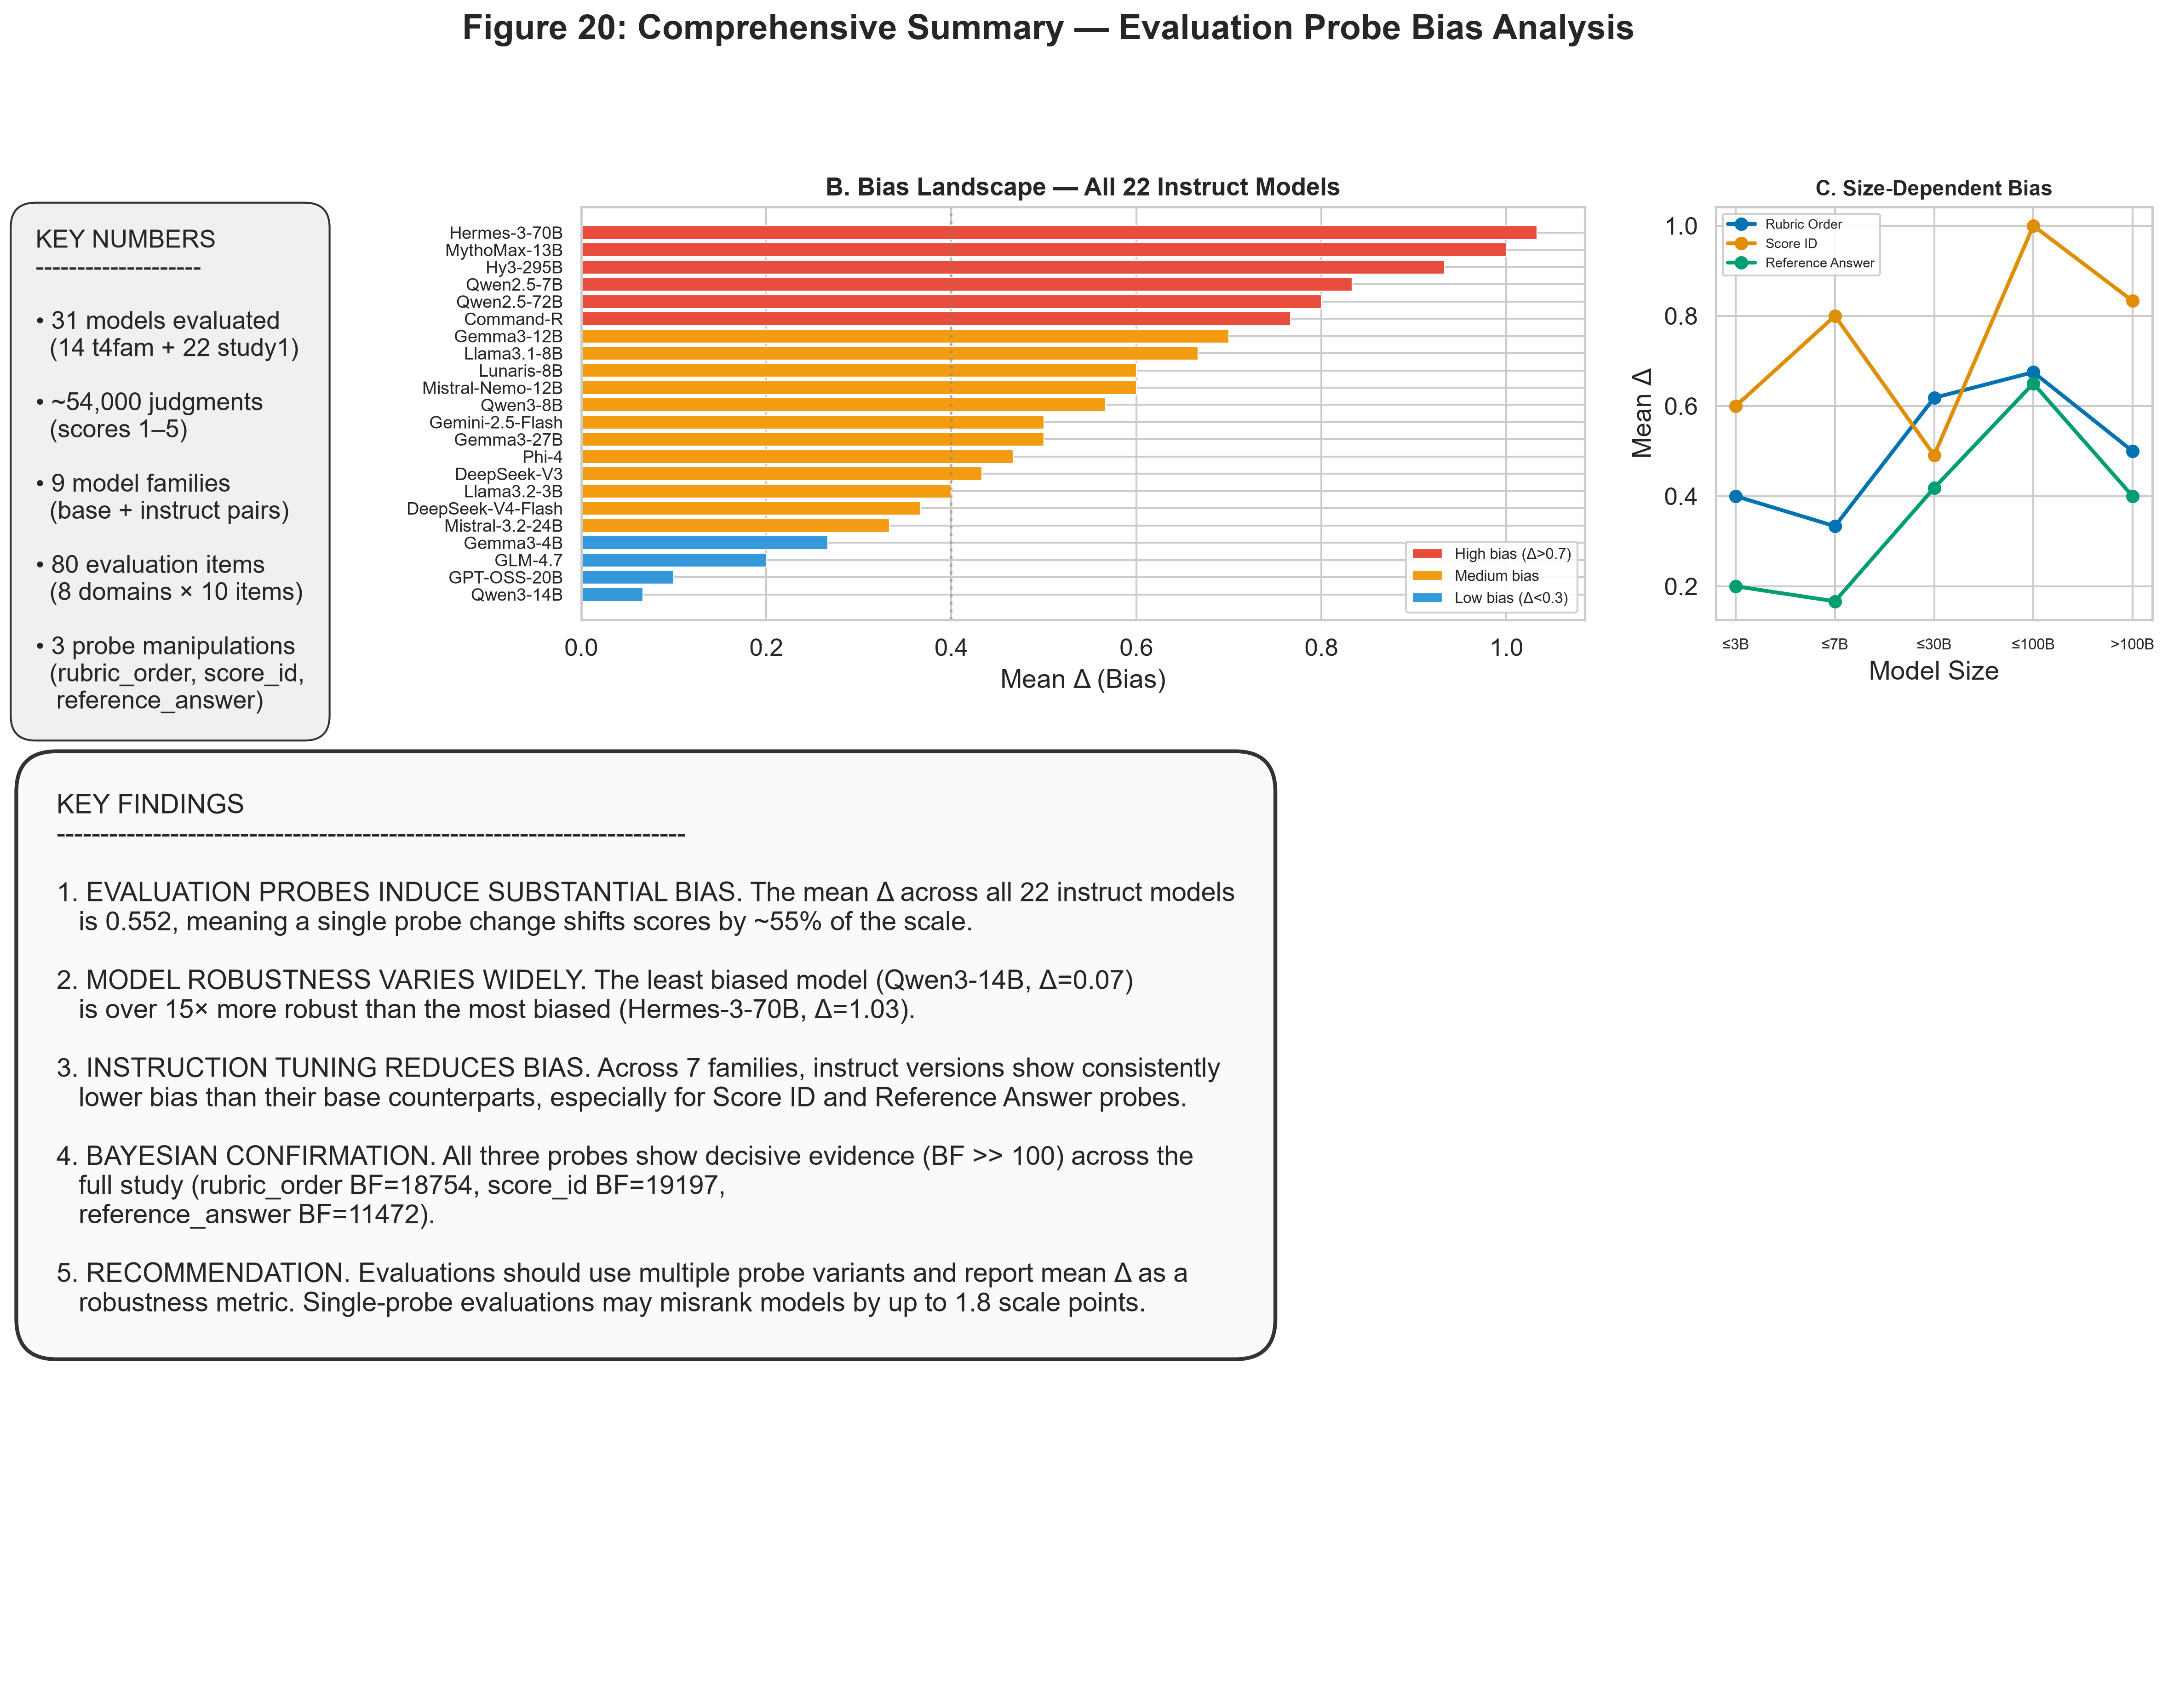
\includegraphics[width=\textwidth]{figures/fig20_comprehensive_summary.png}
\caption{\textbf{Comprehensive research summary.}
This figure integrates four key analyses:
(1) variance decomposition showing between-model vs within-model contributions,
(2) model ranking with color-coded bias levels,
(3) key experimental numbers, and
(4) the five main findings with actionable recommendations.
This multi-panel summary serves as a quick reference for the study's methodology,
results, and practical implications.}
\label{fig:comprehensive_summary}
\end{figure*}
